%===========================================================
% main.tex - 主控文件
%===========================================================
\documentclass[aspectratio=169, 12pt]{beamer}

% 导入配置文件
%===========================================================
% preamble.tex - Beamer 配置文件
%===========================================================

% 中文支持
\usepackage[UTF8]{ctex}

% 图形与表格
\usepackage{graphicx}
\usepackage{booktabs}

% 颜色与图形(必须在listings之前加载)
\usepackage{xcolor}
\usepackage{tikz}
\usetikzlibrary{shapes, arrows.meta, positioning}

% 数学公式
\usepackage{amsmath}
\usepackage{amssymb}

% 代码高亮
\usepackage{listings}

\lstset{
    language=Python,
    basicstyle=\small\ttfamily,
    keywordstyle=\color{blue},
    commentstyle=\color{green!60!black},
    stringstyle=\color{orange},
    breaklines=true,
    showstringspaces=false,
    keepspaces=true
}

% 超链接
\usepackage{hyperref}

%===========================================================
% 主题设置
%===========================================================
\usetheme{Madrid}
\usecolortheme{whale}
\usefonttheme{professionalfonts}

%===========================================================
% 课程信息
%===========================================================
\title[核心开发与调试]{第10周:核心开发与调试}
\subtitle{让系统真正跑起来}
\author{北京石油化工学院\textbackslash 人工智能研究院\textbackslash 王文通}
\institute{通选课}
\date{2025-2026 学年}

%===========================================================
% 自定义命令
%===========================================================
% 高亮命令
\newcommand{\highlight}[1]{\textcolor{red}{\textbf{#1}}}


% 学校信息(包含 logo 图片)
\institute{%
    \raisebox{-0.5cm}{\includegraphics[height=1.2cm]{../name.png}}\hspace{0.5cm}%
    \raisebox{-0.5cm}{\includegraphics[height=1.2cm]{../xiaohui.png}}\hspace{0.3cm}%
    \begin{minipage}{6cm}
        \centering
        \textbf{北京石油化工学院}\\
        \textit{人工智能研究院}
    \end{minipage}
}

\begin{document}

%===========================================================
% 标题页与目录
%===========================================================
\begin{frame}
    \titlepage
\end{frame}

\section*{课程概览}
\begin{frame}{课程概览}
    \begin{columns}
        \column{0.45\textwidth}
        \textbf{本周内容:}
        \begin{itemize}
            \item 手写识别概述
            \item PaddleOCR手写识别
            \item TrOCR高精度识别
            \item 图像预处理优化
            \item 思考题与作业
        \end{itemize}

        \column{0.55\textwidth}
        \textbf{学期项目:AI阅卷助手}
        \begin{enumerate}
            \item 图像采集与预处理
            \item 答题卡定位(Timing Marks)
            \item 填涂检测与识别
            \item 手写文字 OCR(本周重点)
            \item 成绩统计与输出
        \end{enumerate}
    \end{columns}
\end{frame}

\begin{frame}{本周时间分配(160分钟 = 3学时)}
    \begin{columns}
        \column{0.5\textwidth}
        \textbf{第1学时(45分钟):}
        \begin{itemize}
            \item[00:00-00:15] 手写识别概述(15min)
            \item[00:15-00:35] PaddleOCR手写识别(20min)
            \item[00:35-00:45] 讨论与答疑(10min)
        \end{itemize}

        \textbf{第2学时(45分钟):}
        \begin{itemize}
            \item[00:45-01:15] TrOCR高精度识别(30min)
            \item[01:15-01:30] 图像预处理优化(15min)
        \end{itemize}

        \column{0.5\textwidth}
        \textbf{第3学时(70分钟):}
        \begin{itemize}
            \item[01:30-02:00] 代码实战:手写识别(30min)
            \item[02:00-02:20] 参数调优实践(20min)
            \item[02:20-02:35] 互动测验(15min)
            \item[02:35-02:45] 总结与作业(10min)
        \end{itemize}

        \vspace{0.5cm}
        \begin{alertblock}{时间控制提示}
        如果进度落后,建议跳过"挑战任务"
        \end{alertblock}
    \end{columns}
\end{frame}

\begin{frame}{预备知识(课前5分钟视频)}
    \begin{columns}
        \column{0.5\textwidth}
        \textbf{视频1:神经网络基础(2分钟)}

        \vspace{0.2cm}

        \textbf{神经元模型:}
        \begin{itemize}
            \item 模拟人脑神经元
            \item 输入→加权和→激活→输出
            \item 可学习的权重和偏置
        \end{itemize}

        \vspace{0.2cm}

        \textbf{神经网络层次:}
        \begin{itemize}
            \item 输入层:接收数据
            \item 隐藏层:特征提取
            \item 输出层:产生结果
        \end{itemize}

        \column{0.5\textwidth}
        \textbf{视频2:卷积运算直观理解(3分钟)}

        \vspace{0.2cm}

        \textbf{什么是卷积?}
        \begin{itemize}
            \item 滑动窗口提取特征
            \item 卷积核(滤波器)
            \item 特征图(Feature Map)
        \end{itemize}

        \vspace{0.2cm}

        \textbf{卷积在手写识别中的作用:}
        \begin{itemize}
            \item 提取笔画特征
            \item 捕获局部结构
            \item 平移不变性
        \end{itemize}

        \vspace{0.2cm}

        \textbf{常见卷积操作:}
        \begin{itemize}
            \item Valid卷积:尺寸减小
            \item Same卷积:保持尺寸
            \item 池化(Pooling):下采样
        \end{itemize}
    \end{columns}

    \vspace{0.5cm}

    \begin{alertblock}{课前测试}
        观看视频后,请回答:
        \begin{enumerate}
            \item 神经网络的基本单元是什么?
            \item 卷积运算有什么特点?
            \item 卷积在手写识别中起什么作用?
        \end{enumerate}
    \end{alertblock}
\end{frame}

\begin{frame}{本周分组策略}
    \textbf{分组原则:}
    \begin{itemize}
        \item 每4人为一组
        \item 确保不同专业背景混合
        \item 建议包含:理工科、文科、无编程基础、有编程基础
    \end{itemize}

    \vspace{0.3cm}

    \textbf{角色分工:}
    \begin{table}
        \centering
        \small
        \begin{tabular}{lp{6cm}l}
            \toprule
            \textbf{角色} & \textbf{职责} & \textbf{适合} \\
            \midrule
            组长 & 统筹协调、进度管理 & 组织能力强的 \\
            算法实现者 & 实现OCR代码、模型调用 & 有编程基础的 \\
            参数调优者 & 调整识别参数、优化效果 & 细心负责的 \\
            测试者 & 收集测试用例、报告问题 & 细心负责的 \\
            \bottomrule
        \end{tabular}
    \end{table}

    \vspace{0.3cm}

    \begin{block}{本周协作任务}
        实现手写文字识别,对比PaddleOCR和TrOCR效果
    \end{block}
\end{frame}

\begin{frame}{本周在智能阅卷系统中的位置}
    \begin{columns}
        \column{0.5\textwidth}
        \textbf{已完成模块:}
        \begin{enumerate}
            \item \textcolor{green!60!black}{✓} 图像预处理(第3周)
            \item \textcolor{green!60!black}{✓} 版面分析(第4周)
            \item \textcolor{green!60!black}{✓} 选择题识别(第5周)
            \item \textcolor{green!60!black}{✓} 判断题识别(第6周)
            \item \textcolor{green!60!black}{✓} 印刷文字识别(第7周)
        \end{enumerate}

        \vspace{0.3cm}

        \textbf{本周目标:}
        \begin{itemize}
            \item \textcolor{blue}{🔄} 识别手写简答答案
            \item \textcolor{blue}{🔄} 对比PaddleOCR vs TrOCR
            \item \textcolor{blue}{🔄} 优化预处理参数
        \end{itemize}

        \column{0.5\textwidth}
        \textbf{智能阅卷流程:}

        \vspace{0.2cm}

        \begin{center}
            \begin{tikzpicture}[
                node distance=0.4cm,
                box/.style={rectangle, draw=black, minimum width=1.8cm, minimum height=0.5cm, font=\scriptsize, rounded corners},
                arrow/.style={->, thick},
                current/.style={rectangle, draw=blue, fill=blue!20, minimum width=1.8cm, minimum height=0.5cm, font=\scriptsize, rounded corners}
            ]
                \node[box] (p1) {预处理};
                \node[box, right=0.05cm of p1] (p2) {版面};
                \node[box, right=0.05cm of p2] (p3) {选/判};
                \node[box, right=0.05cm of p3] (p4) {印刷};
                \node[current, right=0.05cm of p4] (p5) {手写};
                \node[box, dashed, right=0.05cm of p5] (p6) {评分};

                \draw[arrow] (p1) -- (p2);
                \draw[arrow] (p2) -- (p3);
                \draw[arrow] (p3) -- (p4);
                \draw[arrow] (p4) -- (p5);
                \draw[arrow] (p5) -- (p6);
            \end{tikzpicture}
        \end{center}

        \vspace{0.3cm}

        \textit{\textcolor{blue}{从"印刷文字"到"手写文字"的跨越}}
    \end{columns}

    \vspace{0.5cm}

    \begin{block}{手写识别在智能阅卷中的作用}
        \begin{itemize}
            \item \textbf{简答题自动识别}:将学生手写答案转换为可编辑文本
            \item \textbf{关键词提取}:从手写答案中提取关键信息
            \item \textbf{辅助评分}:为教师提供参考,加快批改速度
            \item \textbf{答案存档}:数字化保存学生手写答案
        \end{itemize}
    \end{block}
\end{frame}

\begin{frame}{多屏协同设计}
    \textbf{本课程采用多屏协同教学方式:}

    \vspace{0.3cm}

    \begin{columns}
        \column{0.5\textwidth}
        \textbf{主屏(左侧):理论讲解}
        \begin{itemize}
            \item PPT幻灯片
            \item 概念和原理讲解
            \item 图像和代码展示
            \item 互动测验
        \end{itemize}

        \column{0.5\textwidth}
        \textbf{侧屏(右侧):实时演示}
        \begin{itemize}
            \item OCR代码实时演示
            \item 手写识别效果展示
            \item 参数调整实时反馈
            \item 调试过程展示
        \end{itemize}
    \end{columns}

    \vspace{0.5cm}

    \begin{block}{移动设备互动}
        使用手机参与互动测验(问卷星)
    \end{block}
\end{frame}

%===========================================================
% 教学模块
%===========================================================
%===========================================================
% 01_overview.tex - 版面分析概述与流程
%===========================================================

\section{版面分析概述}

\begin{frame}{什么是版面分析?}
    \begin{block}{定义}
        从文档图像中识别和定位不同区域(标题、正文、表格、图片等)
    \end{block}

    \vspace{0.3cm}

    \textbf{在阅卷系统中的作用:}
    \begin{enumerate}
        \item 找到试卷边界(定位试卷)
        \item 定位选择题区域(OMR识别)
        \item 定位判断题区域(符号匹配)
        \item 定位简答题区域(手写识别)
        \item 定位填空题区域(内容提取)
    \end{enumerate}
\end{frame}

\begin{frame}{为什么需要版面分析?}
    \begin{columns}
        \column{0.5\textwidth}
        \textbf{没有版面分析:}
        \begin{itemize}
            \item 不知道答题卡在哪
            \item 无法区分题型
            \item OCR识别范围过大
            \item 处理效率低下
        \end{itemize}

        \column{0.5\textwidth}
        \textbf{有了版面分析:}
        \begin{itemize}
            \item 精确定位各区域
            \item 分类处理不同题型
            \item 提高识别准确率
            \item 加快处理速度
        \end{itemize}
    \end{columns}

    \vspace{0.5cm}

    \begin{alertblock}{核心价值}
        版面分析是自动阅卷的"地图导航"!
    \end{alertblock}
\end{frame}

\begin{frame}{版面分析完整流程}
    \begin{center}
        \begin{tikzpicture}[node distance=1.5cm, auto,
            block/.style={draw, rectangle, rounded corners, fill=blue!10, minimum height=0.8cm, minimum width=2cm},
            arrow/.style={->, thick}]

            \node[block] (input) {输入图像};
            \node[block, right of=input, node distance=2.2cm, fill=yellow!10] (pre) {预处理};
            \node[block, right of=pre, node distance=2.2cm, fill=green!10] (edge) {边缘检测};
            \node[block, right of=edge, node distance=2.2cm, fill=red!10] (contour) {轮廓检测};
            \node[block, below of=contour, node distance=1.5cm, fill=purple!10] (filter) {轮廓筛选};
            \node[block, left of=filter, node distance=2.2cm, fill=orange!10] (layout) {版面分析};
            \node[block, left of=layout, node distance=2.2cm, fill=cyan!10] (output) {区域输出};

            \draw[arrow] (input) -- (pre);
            \draw[arrow] (pre) -- (edge);
            \draw[arrow] (edge) -- (contour);
            \draw[arrow] (contour) -- (filter);
            \draw[arrow] (filter) -- (layout);
            \draw[arrow] (layout) -- (output);
        \end{tikzpicture}
    \end{center}
\end{frame}

\begin{frame}{版面分析方法分类}
    \textbf{传统方法:}
    \begin{itemize}
        \item \textbf{边缘检测}:Canny、Sobel
        \item \textbf{轮廓检测}:findContours
        \item \textbf{投影法}:水平/垂直投影
        \item \textbf{连通域分析}:blob检测
    \end{itemize}

    \vspace{0.3cm}

    \textbf{深度学习方法:}
    \begin{itemize}
        \item \textbf{目标检测}:YOLO、Faster R-CNN
        \item \textbf{语义分割}:U-Net、DeepLab
        \item \textbf{版面分析模型}:LayoutLM、DocFormer
    \end{itemize}

    \vspace{0.3cm}

    \begin{block}{本课程重点}
        传统方法(简单、高效、可控)
    \end{block}
\end{frame}

\begin{frame}{应用场景}
    \begin{columns}
        \column{0.33\textwidth}
        \begin{block}{教育阅卷}
            \begin{itemize}
                \item 答题卡识别
                \item 试卷自动批改
                \item 成绩统计
            \end{itemize}
        \end{block}

        \column{0.33\textwidth}
        \begin{block}{文档处理}
            \begin{itemize}
                \item 发票识别
                \item 表单提取
                \item 合同分析
            \end{itemize}
        \end{block}

        \column{0.33\textwidth}
        \begin{block}{档案数字化}
            \begin{itemize}
                \item 版面重建
                \item 区域提取
                \item 内容索引
            \end{itemize}
        \end{block}
    \end{columns}
\end{frame}

%===========================================================
% 02_paddleocr.tex - PaddleOCR手写识别
%===========================================================

\section{PaddleOCR手写识别}

\begin{frame}{PaddleOCR架构概述}
    \begin{columns}
        \begin{column}{0.55\textwidth}
            \textbf{PP-OCRv4三大核心模块}
            \vspace{0.3cm}

            \begin{enumerate}
                \item \textbf{文本检测} (Text Detection)
                \begin{itemize}
                    \item DBNet算法
                    \item 可微分二值化
                \end{itemize}

                \item \textbf{方向分类} (Orientation Classification)
                \begin{itemize}
                    \item 0/90/180/270度分类
                    \item 轻量级CNN
                \end{itemize}

                \item \textbf{文本识别} (Text Recognition)
                \begin{itemize}
                    \item SVTR\_LCNet架构
                    \item CTC解码
                \end{itemize}
            \end{enumerate}
        \end{column}
        \begin{column}{0.43\textwidth}
            \begin{tikzpicture}[
                node distance=0.6cm,
                box/.style={draw, rounded corners, fill=blue!10, minimum width=3.5cm, minimum height=0.7cm, align=center, font=\small}
            ]
                \node[box] (input) {输入图像};
                \node[box, below=of input, fill=red!10] (det) {文本检测\\DBNet};
                \node[box, below=of det, fill=yellow!10] (cls) {方向分类\\CNN};
                \node[box, below=of cls, fill=green!10] (rec) {文本识别\\SVTR};
                \node[box, below=of rec] (output) {识别结果};

                \draw[->, thick] (input) -- (det);
                \draw[->, thick] (det) -- (cls);
                \draw[->, thick] (cls) -- (rec);
                \draw[->, thick] (rec) -- (output);
            \end{tikzpicture}
        \end{column}
    \end{columns}
\end{frame}

\begin{frame}{检测模型:DBNet原理}
    \begin{columns}
        \begin{column}{0.5\textwidth}
            \textbf{DBNet (Differentiable Binarization)}

            \vspace{0.3cm}
            \textbf{核心创新:可微分二值化}
            \begin{itemize}
                \item 传统方法:二值化不可导,无法端到端训练
                \item DBNet:将二值化近似为可微分函数
                \item 梯度可直接传播到阈值预测
            \end{itemize}

            \vspace{0.3cm}
            \textbf{二值化公式:}
            \[
            B_{i,j} = \frac{1}{1 + e^{-k(P_{i,j} - T_{i,j})}}
            \]
            其中:$P$为概率图,$T$为阈值图,$k$为放大因子
        \end{column}
        \begin{column}{0.48\textwidth}
            \begin{tikzpicture}[
                node distance=0.4cm,
                smallbox/.style={draw, rounded corners, fill=blue!10, minimum width=4cm, minimum height=0.6cm, align=center, font=\small}
            ]
                \node[smallbox] (input) {输入图像};
                \node[smallbox, below=of input] (backbone) {Backbone (ResNet)};
                \node[smallbox, below=of backbone] (neck) {FPN (特征融合)};
                \node[smallbox, below=of neck, fill=green!10] (prob) {概率图 $P$};
                \node[smallbox, below=of prob, fill=yellow!10] (thresh) {阈值图 $T$};
                \node[smallbox, below=of thresh, fill=red!10] (binary) {近似二值图 $\hat{B}$};

                \draw[->, thick] (input) -- (backbone);
                \draw[->, thick] (backbone) -- (neck);
                \draw[->, thick] (neck) -- (prob);
                \draw[->, thick] (neck) -- (thresh);
                \draw[->, thick] (prob) -- (binary);
                \draw[->, thick] (thresh) -- (binary);
            \end{tikzpicture}
        \end{column}
    \end{columns}
\end{frame}

\begin{frame}{识别模型:SVTR\_LCNet原理}
    \begin{columns}
        \begin{column}{0.5\textwidth}
            \textbf{SVTR\_LCNet架构}

            \vspace{0.3cm}
            \textbf{设计目标:}
            \begin{itemize}
                \item 中文场景文字识别
                \item 支持横排和竖排文本
                \item 平衡精度与速度
            \end{itemize}

            \vspace{0.3cm}
            \textbf{网络结构:}
            \begin{enumerate}
                \item \textbf{LCNet骨干网络}
                \begin{itemize}
                    \item 轻量级CNN架构
                    \item 深度可分离卷积
                \end{itemize}
                \item \textbf{SVTR编码器}
                \begin{itemize}
                    \item 基于Sub-Block的Transformer
                    \item 全局特征建模
                \end{itemize}
                \item \textbf{CTC解码器}
                \begin{itemize}
                    \item 无需字符级对齐
                    \item 处理不定长序列
                \end{itemize}
            \end{enumerate}
        \end{column}
        \begin{column}{0.48\textwidth}
            \begin{tikzpicture}[
                node distance=0.35cm,
                box/.style={draw, rounded corners, minimum width=4cm, minimum height=0.55cm, align=center, font=\small}
            ]
                \node[box, fill=blue!10] (input) {输入图像 (H×W×C)};
                \node[box, below=of input, fill=cyan!10] (lcnet) {LCNet骨干网络};
                \node[box, below=of lcnet, fill=green!10] (feature) {特征图 (H'×W'×C')};
                \node[box, below=of feature, fill=yellow!10] (svtr) {SVTR编码器};
                \node[box, below=of svtr, fill=orange!10] (seq) {序列特征 (T×D)};
                \node[box, below=of seq, fill=red!10] (ctc) {CTC解码器};
                \node[box, below=of ctc, fill=purple!10] (output) {识别结果};

                \draw[->, thick] (input) -- (lcnet);
                \draw[->, thick] (lcnet) -- (feature);
                \draw[->, thick] (feature) -- (svtr);
                \draw[->, thick] (svtr) -- (seq);
                \draw[->, thick] (seq) -- (ctc);
                \draw[->, thick] (ctc) -- (output);
            \end{tikzpicture}

            \vspace{0.5cm}
            \textbf{CTC解码公式:}
            \[
            p(l|x) = \sum_{\pi \in B^{-1}(l)} p(\pi|x)
            \]
        \end{column}
    \end{columns}
\end{frame}

\begin{frame}[fragile]{PaddleOCR手写配置}
    \begin{lstlisting}
from paddleocr import PaddleOCR

# TODO: 使用AI助手补全PaddleOCR初始化
# 提示词:"PaddleOCR手写识别配置参数说明"
ocr_handwrite = PaddleOCR(
    use_angle_cls=______,  # TODO: 是否启用方向分类(True/False)
    lang=______,           # TODO: 语言设置('ch'/'en'/...)
    show_log=______        # TODO: 是否显示日志(True/False)
)

# TODO: 调用OCR识别方法
# 提示词:"PaddleOCR ocr()方法参数说明"
result = ocr_handwrite.ocr(
    ______,  # TODO: 输入图像路径或数组
    cls=______  # TODO: 是否启用方向分类(True/False)
)

# TODO: 解析并打印识别结果
# 提示词:"PaddleOCR识别结果结构解析"
for line in result:
    text = ______  # TODO: 提取文字内容
    confidence = ______  # TODO: 提取置信度
    print(f"{text} ({confidence:.4f})")
    \end{lstlisting}

    \textbf{注意:} PaddleOCR默认已支持手写识别
\end{frame}

\begin{frame}[fragile]{手写识别参数调优}
    \begin{lstlisting}
# TODO: 使用AI助手补全手写识别优化配置
# 提示词:"PaddleOCR手写识别参数调优指南"
ocr_optimized = PaddleOCR(
    use_angle_cls=______,  # TODO: 是否启用方向分类
    lang=______,           # TODO: 语言设置
    # TODO: 模型路径配置
    det_model_dir=______,  # TODO: 检测模型路径
    rec_model_dir=______,  # TODO: 识别模型路径
    cls_model_dir=______,  # TODO: 方向分类模型路径
    # TODO: 性能参数调优
    rec_batch_num=______,   # TODO: 批量识别数(整数)
    max_text_length=______, # TODO: 最大文本长度(整数)
    drop_score=______,      # TODO: 置信度阈值(0-1浮点数)
    show_log=______         # TODO: 是否显示日志
)
    \end{lstlisting}
\end{frame}

\begin{frame}[fragile]{多行手写文字识别}
    \begin{lstlisting}
import cv2
from paddleocr import PaddleOCR

# TODO: 使用AI助手补全图像读取代码
# 提示词:"OpenCV读取图像的常用方法"
image = cv2.______  # TODO: 读取图像文件(如'answer_sheet.jpg')

# TODO: 初始化OCR
# 提示词:"PaddleOCR初始化参数说明"
ocr = PaddleOCR(
    use_angle_cls=______,  # TODO: 是否启用方向分类
    lang=______           # TODO: 语言设置
)

# TODO: 执行OCR识别
result = ocr.ocr(
    ______,  # TODO: 输入图像
    cls=______  # TODO: 是否启用方向分类
)

# TODO: 提取文字块并按位置排序
# 提示词:"如何根据边界框坐标对OCR结果排序"
text_blocks = []
for line in result[0]:
    box = ______  # TODO: 提取边界框坐标
    text = ______  # TODO: 提取文字内容
    conf = ______  # TODO: 提取置信度
    # TODO: 计算中心点y坐标
    center_y = ______  # TODO: 计算边界框中心y坐标
    text_blocks.append((center_y, text, conf))

# TODO: 按y坐标排序(从上到下)
text_blocks.sort(key=______)
    \end{lstlisting}
\end{frame}

\begin{frame}[fragile]{增强版手写识别(含错误处理)}
    \begin{lstlisting}
import os
import cv2
import numpy as np
from paddleocr import PaddleOCR
from typing import List, Dict, Optional, Union

class HandwritingOCR:
    """增强版手写OCR识别器"""

    def __init__(self,
                 use_gpu: bool = False,
                 det_model_dir: Optional[str] = None,
                 rec_model_dir: Optional[str] = None,
                 drop_score: float = 0.3):
        """
        初始化OCR识别器

        Args:
            use_gpu: 是否使用GPU
            det_model_dir: 检测模型路径
            rec_model_dir: 识别模型路径
            drop_score: 置信度过滤阈值
        """
        try:
            self.ocr = PaddleOCR(
                use_angle_cls=True,
                lang='ch',
                use_gpu=use_gpu,
                det_model_dir=det_model_dir,
                rec_model_dir=rec_model_dir,
                drop_score=drop_score,
                show_log=False
            )
            self.drop_score = drop_score
            print("[INFO] OCR模型初始化成功")
        except Exception as e:
            raise RuntimeError(f"OCR初始化失败: {str(e)}")
    \end{lstlisting}
\end{frame}

\begin{frame}[fragile]{批量处理与结果可视化}
    \begin{lstlisting}
    def batch_recognize(self,
                       image_paths: List[str],
                       save_results: bool = True,
                       output_dir: str = "./results") -> List[Dict]:
        """
        批量识别手写文字

        Args:
            image_paths: 图像路径列表
            save_results: 是否保存可视化结果
            output_dir: 输出目录

        Returns:
            识别结果列表,每项包含:
            - image_path: 图像路径
            - texts: 识别文字列表
            - confidences: 置信度列表
            - avg_confidence: 平均置信度
        """
        if save_results and not os.path.exists(output_dir):
            os.makedirs(output_dir)

        results = []
        for img_path in image_paths:
            if not os.path.exists(img_path):
                print(f"[WARN] 文件不存在: {img_path}")
                continue

            try:
                result = self.recognize_single(img_path,
                                               save_vis=save_results,
                                               output_dir=output_dir)
                results.append(result)
            except Exception as e:
                print(f"[ERROR] 处理 {img_path} 失败: {str(e)}")

        return results
    \end{lstlisting}
\end{frame}

\begin{frame}[fragile]{单张图像识别与可视化}
    \begin{lstlisting}
    def recognize_single(self,
                        image_path: str,
                        save_vis: bool = True,
                        output_dir: str = "./results") -> Dict:
        """
        单张图像手写文字识别

        Args:
            image_path: 图像路径
            save_vis: 是否保存可视化结果
            output_dir: 输出目录

        Returns:
            识别结果字典
        """
        # 读取图像
        image = cv2.imread(image_path)
        if image is None:
            raise ValueError(f"无法读取图像: {image_path}")

        # 执行OCR识别
        ocr_result = self.ocr.ocr(image_path, cls=True)

        # 解析结果
        texts = []
        confidences = []
        boxes = []

        if ocr_result and ocr_result[0]:
            for line in ocr_result[0]:
                box = line[0]  # 边界框坐标
                text = line[1][0]  # 识别文本
                conf = line[1][1]  # 置信度

                # 过滤低置信度结果
                if conf >= self.drop_score:
                    boxes.append(box)
                    texts.append(text)
                    confidences.append(conf)

        # 按位置排序(从上到下)
        if boxes:
            sorted_data = sorted(zip(boxes, texts, confidences),
                                key=lambda x: (x[0][0][1] + x[0][2][1]) / 2)
            boxes, texts, confidences = zip(*sorted_data) if sorted_data else ([], [], [])

        # 可视化结果
        vis_image = None
        if save_vis:
            vis_image = self._visualize_result(image, boxes, texts, confidences)
            output_path = os.path.join(output_dir, f"vis_{os.path.basename(image_path)}")
            cv2.imwrite(output_path, vis_image)
            print(f"[INFO] 可视化结果已保存: {output_path}")

        # 计算平均置信度
        avg_conf = sum(confidences) / len(confidences) if confidences else 0.0

        return {
            'image_path': image_path,
            'texts': list(texts),
            'confidences': list(confidences),
            'avg_confidence': avg_conf,
            'boxes': list(boxes),
            'visualization': vis_image
        }
    \end{lstlisting}
\end{frame}

\begin{frame}[fragile]{结果可视化方法}
    \begin{lstlisting}
    def _visualize_result(self,
                         image: np.ndarray,
                         boxes: List[List],
                         texts: List[str],
                         confidences: List[float],
                         box_color: Tuple[int, int, int] = (0, 255, 0),
                         text_color: Tuple[int, int, int] = (255, 0, 0)) -> np.ndarray:
        """
        可视化识别结果

        Args:
            image: 原始图像
            boxes: 边界框列表
            texts: 识别文本列表
            confidences: 置信度列表
            box_color: 框颜色 (BGR)
            text_color: 文字颜色 (BGR)

        Returns:
            可视化后的图像
        """
        vis_image = image.copy()

        for i, (box, text, conf) in enumerate(zip(boxes, texts, confidences)):
            # 绘制边界框
            box_pts = np.array(box, dtype=np.int32).reshape((-1, 1, 2))
            cv2.polylines(vis_image, [box_pts], True, box_color, 2)

            # 准备显示文本
            display_text = f"{text} ({conf:.2f})"

            # 计算文本位置(框的左上角)
            text_pos = (int(box[0][0]), int(box[0][1]) - 5)

            # 获取文本大小以绘制背景
            (text_w, text_h), _ = cv2.getTextSize(
                display_text, cv2.FONT_HERSHEY_SIMPLEX, 0.5, 2
            )

            # 绘制文本背景
            cv2.rectangle(
                vis_image,
                (text_pos[0], text_pos[1] - text_h - 4),
                (text_pos[0] + text_w, text_pos[1] + 4),
                (0, 0, 0),
                -1
            )

            # 绘制文本
            cv2.putText(
                vis_image, display_text, text_pos,
                cv2.FONT_HERSHEY_SIMPLEX, 0.5, text_color, 2
            )

        return vis_image


# 使用示例
if __name__ == "__main__":
    # 初始化OCR
    ocr = HandwritingOCR(use_gpu=False, drop_score=0.3)

    # 单张识别
    result = ocr.recognize_single("handwriting.jpg", save_vis=True)
    print(f"识别结果: {result['texts']}")
    print(f"平均置信度: {result['avg_confidence']:.4f}")
    \end{lstlisting}
\end{frame}

% 注意:重复的PaddleOCR配置页面已删除,相关内容见上方"PaddleOCR手写配置"和"手写识别参数调优"页面

%===========================================================
% 03_trocr.tex - TrOCR高精度识别
%===========================================================

\section{TrOCR高精度识别}

\begin{frame}{TrOCR简介}
    \textbf{TrOCR:} Transformer-based OCR

    \begin{itemize}
        \item 开发者:Microsoft
        \item 架构:ViT (图像编码器) + GPT-2 (文本解码器)
        \item 优势:端到端训练,准确率最高
    \end{itemize}

    \vspace{0.3cm}

    \textbf{模型:}
    \begin{itemize}
        \item trocr-base-handwritten
        \item trocr-large-handwritten
    \end{itemize}
\end{frame}

%-----------------------------------------------------------
% 新增:Transformer架构基础
%-----------------------------------------------------------

\begin{frame}{Transformer架构概述}
    \textbf{Transformer}是一种完全基于注意力机制的序列转换模型

    \begin{center}
    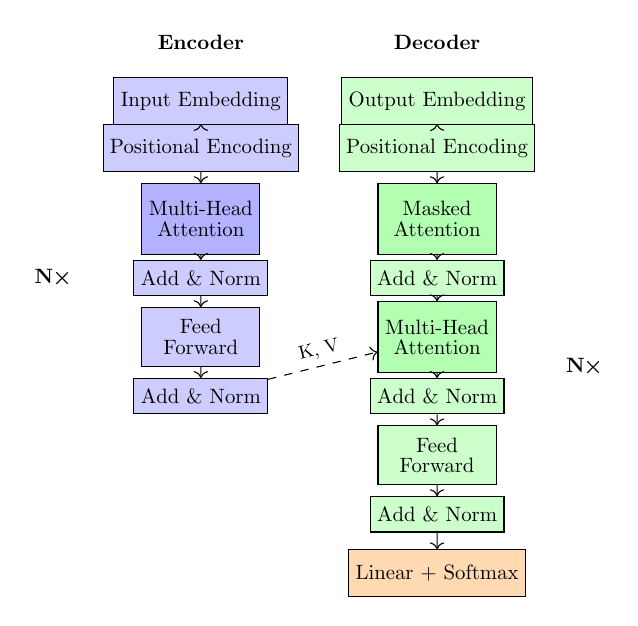
\begin{tikzpicture}[scale=0.75, transform shape]
        % Encoder
        \node[draw, fill=blue!20, minimum width=2cm, minimum height=0.8cm] (enc1) at (0,3) {Input Embedding};
        \node[draw, fill=blue!20, minimum width=2cm, minimum height=0.8cm] (pos1) at (0,2.2) {Positional Encoding};
        \node[draw, fill=blue!30, minimum width=2cm, minimum height=1.2cm] (enc2) at (0,1) {\shortstack{Multi-Head\\Attention}};
        \node[draw, fill=blue!20, minimum width=2cm, minimum height=0.6cm] (norm1) at (0,0) {Add \& Norm};
        \node[draw, fill=blue!20, minimum width=2cm, minimum height=1cm] (ffn) at (0,-1) {\shortstack{Feed\\Forward}};
        \node[draw, fill=blue!20, minimum width=2cm, minimum height=0.6cm] (norm2) at (0,-2) {Add \& Norm};

        % Decoder
        \node[draw, fill=green!20, minimum width=2cm, minimum height=0.8cm] (dec1) at (4,3) {Output Embedding};
        \node[draw, fill=green!20, minimum width=2cm, minimum height=0.8cm] (pos2) at (4,2.2) {Positional Encoding};
        \node[draw, fill=green!30, minimum width=2cm, minimum height=1.2cm] (dec2) at (4,1) {\shortstack{Masked\\Attention}};
        \node[draw, fill=green!20, minimum width=2cm, minimum height=0.6cm] (norm3) at (4,0) {Add \& Norm};
        \node[draw, fill=green!30, minimum width=2cm, minimum height=1.2cm] (dec3) at (4,-1) {\shortstack{Multi-Head\\Attention}};
        \node[draw, fill=green!20, minimum width=2cm, minimum height=0.6cm] (norm4) at (4,-2) {Add \& Norm};
        \node[draw, fill=green!20, minimum width=2cm, minimum height=1cm] (ffn2) at (4,-3) {\shortstack{Feed\\Forward}};
        \node[draw, fill=green!20, minimum width=2cm, minimum height=0.6cm] (norm5) at (4,-4) {Add \& Norm};

        % Output
        \node[draw, fill=orange!30, minimum width=2cm, minimum height=0.8cm] (out) at (4,-5) {Linear + Softmax};

        % Arrows encoder
        \draw[->] (enc1) -- (pos1);
        \draw[->] (pos1) -- (enc2);
        \draw[->] (enc2) -- (norm1);
        \draw[->] (norm1) -- (ffn);
        \draw[->] (ffn) -- (norm2);

        % Arrows decoder
        \draw[->] (dec1) -- (pos2);
        \draw[->] (pos2) -- (dec2);
        \draw[->] (dec2) -- (norm3);
        \draw[->] (norm3) -- (dec3);
        \draw[->] (dec3) -- (norm4);
        \draw[->] (norm4) -- (ffn2);
        \draw[->] (ffn2) -- (norm5);
        \draw[->] (norm5) -- (out);

        % Cross attention
        \draw[->, dashed] (norm2) -- (dec3) node[midway, above, sloped, font=\small] {K, V};

        % Labels
        \node[font=\bfseries] at (0,4) {Encoder};
        \node[font=\bfseries] at (4,4) {Decoder};
        \node[font=\bfseries] at (-2.5,0) {N\texttimes};
        \node[font=\bfseries] at (6.5,-1.5) {N\texttimes};
    \end{tikzpicture}
    \end{center}
\end{frame}

\begin{frame}{自注意力机制原理}
    \textbf{自注意力(Self-Attention)}:计算序列中每个位置与其他所有位置的关联强度

    \vspace{0.3cm}

    \textbf{核心公式:}
    $$\text{Attention}(Q, K, V) = \text{softmax}\left(\frac{QK^T}{\sqrt{d_k}}\right)V$$

    \vspace{0.3cm}

    \begin{columns}
        \begin{column}{0.5\textwidth}
            \textbf{Query (Q):}查询向量\\
            \textbf{Key (K):}键向量\\
            \textbf{Value (V):}值向量
        \end{column}
        \begin{column}{0.5\textwidth}
            \begin{itemize}
                \item $QK^T$:计算相似度
                \item $\sqrt{d_k}$:缩放因子
                \item softmax:归一化为概率
                \item 加权求和得到输出
            \end{itemize}
        \end{column}
    \end{columns}
\end{frame}

\begin{frame}{多头注意力机制}
    \textbf{多头注意力(Multi-Head Attention)}:并行计算多组自注意力,捕获不同子空间的信息

    \vspace{0.3cm}

    $$\text{MultiHead}(Q, K, V) = \text{Concat}(\text{head}_1, ..., \text{head}_h)W^O$$

    $$\text{where } \text{head}_i = \text{Attention}(QW_i^Q, KW_i^K, VW_i^V)$$

    \vspace{0.3cm}

    \begin{center}
    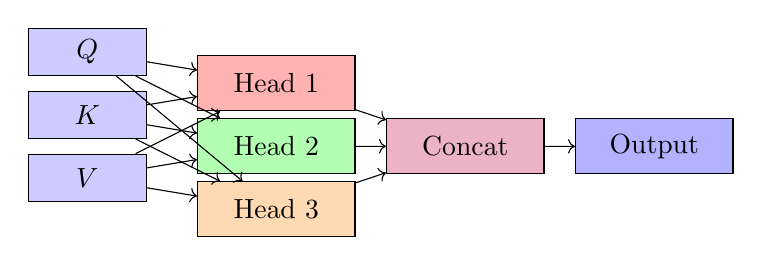
\begin{tikzpicture}[scale=0.8]
        % Input
        \node[draw, fill=blue!20, minimum width=1.5cm, minimum height=0.6cm] (q) at (0,3) {$Q$};
        \node[draw, fill=blue!20, minimum width=1.5cm, minimum height=0.6cm] (k) at (0,2) {$K$};
        \node[draw, fill=blue!20, minimum width=1.5cm, minimum height=0.6cm] (v) at (0,1) {$V$};

        % Heads
        \foreach \i/\y/\c in {1/2.5/red, 2/1.5/green, 3/0.5/orange} {
            \node[draw, fill=\c!30, minimum width=2cm, minimum height=0.7cm] (h\i) at (3,\y) {Head \i};
        }

        % Concat and output
        \node[draw, fill=purple!30, minimum width=2cm, minimum height=0.7cm] (concat) at (6,1.5) {Concat};
        \node[draw, fill=blue!30, minimum width=2cm, minimum height=0.7cm] (out) at (9,1.5) {Output};

        % Arrows
        \foreach \h in {1,2,3} {
            \draw[->] (q) -- (h\h);
            \draw[->] (k) -- (h\h);
            \draw[->] (v) -- (h\h);
            \draw[->] (h\h) -- (concat);
        }
        \draw[->] (concat) -- (out);
    \end{tikzpicture}
    \end{center}
\end{frame}

%-----------------------------------------------------------
% 新增:ViT编码器原理
%-----------------------------------------------------------

\begin{frame}{Vision Transformer (ViT) 架构}
    \textbf{ViT}将Transformer应用于图像分类,TrOCR使用ViT作为图像编码器

    \vspace{0.3cm}

    \textbf{核心思想:}将图像分割成固定大小的块(Patches),将每个块视为一个"词"

    \vspace{0.3cm}

    \begin{center}
    \begin{tikzpicture}[scale=0.7]
        % Original image
        \node at (-3, 2) {原始图像};
        \draw[fill=gray!30] (-4, 0) rectangle (-2, 2);
        \draw[step=0.5] (-4, 0) grid (-2, 2);
        \node at (-3, -0.5) {$224 \times 224$};

        % Arrow
        \draw[->, thick] (-1.5, 1) -- (-0.5, 1) node[midway, above] {分块};

        % Patches
        \node at (2, 2) {图像块序列};
        \foreach \x/\i in {0.5/1, 1.3/2, 2.1/3, 2.9/4, 3.7/5} {
            \draw[fill=blue!20] (\x, 1.2) rectangle (\x+0.6, 1.8);
            \node at (\x+0.3, 1.5) {\tiny $p_\i$};
        }
        \node at (2.5, 0.7) {$\cdots$};

        % Arrow
        \draw[->, thick] (4.5, 1) -- (5.5, 1) node[midway, above] {嵌入};

        % Embeddings
        \node at (7.5, 2) {向量序列};
        \foreach \x/\i in {6.5/1, 7.3/2, 8.1/3, 8.9/4} {
            \draw[fill=green!20] (\x, 1) rectangle (\x+0.6, 1.6);
            \node at (\x+0.3, 1.3) {\tiny $e_\i$};
        }
        \node at (8, 0.5) {$\cdots$};
    \end{tikzpicture}
    \end{center}
\end{frame}

\begin{frame}{ViT编码器结构详解}
    \textbf{ViT编码器的主要组件:}

    \vspace{0.3cm}

    \begin{enumerate}
        \item \textbf{图像分块(Patch Embedding)}
        $$x_p = \text{Flatten}(x_{p}^{(H)} \times x_{p}^{(W)}) \cdot E$$
        其中 $E \in \mathbb{R}^{(P^2 \cdot C) \times D}$ 是可学习的嵌入矩阵

        \vspace{0.2cm}

        \item \textbf{类别Token([CLS] Token)}
        $$z_0 = [x_{\text{class}}; x_p^1E; x_p^2E; \cdots; x_p^NE] + E_{\text{pos}}$$

        \vspace{0.2cm}

        \item \textbf{Transformer编码器层}
        $$z'_{\ell} = \text{MSA}(\text{LN}(z_{\ell-1})) + z_{\ell-1}$$
        $$z_{\ell} = \text{MLP}(\text{LN}(z'_{\ell})) + z'_{\ell}$$
    \end{enumerate}
\end{frame}

\begin{frame}{ViT与CNN编码器对比}
    \begin{columns}
        \begin{column}{0.5\textwidth}
            \textbf{CNN编码器}
            \begin{itemize}
                \item 局部感受野
                \item 平移等变性
                \item 归纳偏置强
                \item 需要大量卷积层提取全局信息
                \item 计算效率高
            \end{itemize}

            \vspace{0.3cm}

            \begin{center}
            \begin{tikzpicture}[scale=0.5]
                \draw[fill=red!20] (0,0) grid (4,4) rectangle (0,0);
                \draw[fill=blue!50] (1,2) rectangle (2,3);
                \node at (0.5, 3.5) {\tiny 局部};
            \end{tikzpicture}
            \end{center}
        \end{column}

        \begin{column}{0.5\textwidth}
            \textbf{ViT编码器}
            \begin{itemize}
                \item 全局感受野
                \item 自注意力机制
                \item 归纳偏置弱
                \item 直接建模全局关系
                \item 数据需求大
            \end{itemize}

            \vspace{0.3cm}

            \begin{center}
            \begin{tikzpicture}[scale=0.5]
                \draw[fill=blue!20] (0,0) grid (4,4) rectangle (0,0);
                \foreach \i in {0,1,2,3} {
                    \foreach \j in {0,1,2,3} {
                        \draw[->, red, thin] (\i+0.5, \j+0.5) -- (2.5, 2.5);
                    }
                }
                \node at (0.5, 3.5) {\tiny 全局};
            \end{tikzpicture}
            \end{center}
        \end{column}
    \end{columns}
\end{frame}

%-----------------------------------------------------------
% 新增:GPT-2解码器原理
%-----------------------------------------------------------

\begin{frame}{GPT-2解码器架构}
    \textbf{GPT-2(Generative Pre-trained Transformer 2)}作为TrOCR的文本解码器

    \vspace{0.3cm}

    \textbf{核心特点:}
    \begin{itemize}
        \item \textbf{仅解码器结构:}使用Masked Self-Attention,只能看到当前位置之前的信息
        \item \textbf{自回归生成:}逐个字符预测,每个新字符依赖于已生成的序列
        \item \textbf{位置编码:}使用可学习的位置嵌入
    \end{itemize}

    \vspace{0.3cm}

    \textbf{解码过程:}
    \begin{align*}
        h_0 &= W_e \cdot x + W_p \\
        h_l &= \text{TransformerBlock}(h_{l-1}), \quad l = 1, \ldots, n \\
        P(y_i | y_{<i}) &= \text{softmax}(W_e^T h_n^{(i)})
    \end{align*}
\end{frame}

\begin{frame}{自回归生成与解码策略}
    \textbf{自回归生成过程:}

    \begin{center}
    \begin{tikzpicture}[scale=0.9, transform shape]
        % Tokens
        \node[draw, fill=green!20, minimum width=1cm, minimum height=0.6cm] (sos) at (0,0) {<sos>};
        \node[draw, fill=blue!20, minimum width=1cm, minimum height=0.6cm] (t1) at (1.5,0) {"H"};
        \node[draw, fill=blue!20, minimum width=1cm, minimum height=0.6cm] (t2) at (3,0) {"e"};
        \node[draw, fill=blue!20, minimum width=1cm, minimum height=0.6cm] (t3) at (4.5,0) {"l"};
        \node[draw, fill=blue!20, minimum width=1cm, minimum height=0.6cm] (t4) at (6,0) {"l"};
        \node[draw, fill=blue!20, minimum width=1cm, minimum height=0.6cm] (t5) at (7.5,0) {"o"};
        \node[draw, fill=red!20, minimum width=1cm, minimum height=0.6cm] (eos) at (9,0) {<eos>};

        % Arrows
        \draw[->] (sos) -- (t1);
        \draw[->] (t1) -- (t2);
        \draw[->] (t2) -- (t3);
        \draw[->] (t3) -- (t4);
        \draw[->] (t4) -- (t5);
        \draw[->] (t5) -- (eos);

        % Model
        \node[draw, fill=gray!30, minimum width=8cm, minimum height=0.8cm] (model) at (4.5,2) {GPT-2 Decoder};

        % Connections to model
        \foreach \x in {0,1.5,3,4.5,6,7.5} {
            \draw[->, gray] (\x,0.5) -- (\x,1.6);
        }

        % Prediction
        \node at (4.5,-1) {每次预测下一个最可能的字符};
    \end{tikzpicture}
    \end{center}

    \vspace{0.3cm}

    \textbf{常用解码策略:}
    \begin{itemize}
        \item \textbf{贪心解码(Greedy):}每次选择概率最高的词
        \item \textbf{束搜索(Beam Search):}保留top-k个候选序列
        \item \textbf{采样解码:}按概率分布随机采样,配合温度参数
    \end{itemize}
\end{frame}

%-----------------------------------------------------------
% 新增:TrOCR训练与微调
%-----------------------------------------------------------

\begin{frame}{TrOCR预训练过程}
    \textbf{TrOCR采用两阶段预训练策略:}

    \vspace{0.3cm}

    \textbf{阶段一:图像编码器预训练(ViT)}
    \begin{itemize}
        \item 数据集:ImageNet-21k
        \item 任务:图像分类
        \item 目标:学习通用的视觉特征表示
    \end{itemize}

    \vspace{0.3cm}

    \textbf{阶段二:端到端文本识别预训练}
    \begin{itemize}
        \item 数据集:
        \begin{itemize}
            \item 合成数据:Synthetically generated handwritten text (数百GB)
            \item 真实数据:IAM, CVL, RIMES等手写数据集
        \end{itemize}
        \item 目标:学习从图像到文本的映射
    \end{itemize}
\end{frame}

\begin{frame}{TrOCR微调方法}
    \textbf{在特定任务上微调TrOCR的常用策略:}

    \vspace{0.3cm}

    \begin{columns}
        \begin{column}{0.55\textwidth}
            \textbf{1. 全模型微调(Full Fine-tuning)}
            \begin{itemize}
                \item 解冻所有参数
                \item 学习率:$5e-6$ 到 $1e-5$
                \item 适合:数据充足的场景
            \end{itemize}

            \vspace{0.3cm}

            \textbf{2. 冻结编码器微调}
            \begin{itemize}
                \item 冻结ViT编码器
                \item 只微调GPT-2解码器
                \item 适合:数据有限的场景
            \end{itemize}
        \end{column}

        \begin{column}{0.45\textwidth}
            \textbf{3. 增量学习}
            \begin{itemize}
                \item 在新数据上继续预训练
                \item 保持原有知识
                \item 逐步适应新领域
            \end{itemize}

            \vspace{0.3cm}

            \textbf{关键超参数:}
            \begin{itemize}
                \item Batch size: 8-32
                \item Epochs: 5-20
                \item Learning rate: $1e-6$ 到 $5e-5$
                \item Warmup steps: 100-500
                \item Weight decay: 0.01
            \end{itemize}
        \end{column}
    \end{columns}
\end{frame}

\begin{frame}{微调数据集准备}
    \textbf{准备用于微调TrOCR的数据集:}

    \vspace{0.3cm}

    \textbf{1. 数据格式}
    \begin{lstlisting}[language=python, basicstyle=\ttfamily\tiny]
# 目录结构
dataset/
  train/
    image_001.jpg
    image_002.jpg
    ...
  val/
    image_101.jpg
    ...
  train_labels.txt  # 格式: 文件名\t文本
  val_labels.txt

# labels.txt 示例
image_001.jpg\t这是一个手写文字示例
image_002.jpg\tHello World
    \end{lstlisting}

    \vspace{0.3cm}

    \textbf{2. 数据增强策略}
    \begin{itemize}
        \item 随机旋转(-5° 到 +5°)
        \item 随机缩放(0.95x 到 1.05x)
        \item 高斯噪声添加
        \item 随机亮度/对比度调整
    \end{itemize}
\end{frame}

%-----------------------------------------------------------
% 原始TrOCR使用代码(保留)
%-----------------------------------------------------------

\begin{frame}[fragile]{TrOCR使用}
    \begin{lstlisting}
# TODO: 使用AI助手补全TrOCR手写识别代码
# 提示词:"使用TrOCR进行手写文字识别的完整流程"
from transformers import TrOCRProcessor, VisionEncoderDecoderModel
from PIL import Image

# TODO: 加载TrOCR处理器和模型
# 提示词:"TrOCRProcessor和VisionEncoderDecoderModel的from_pretrained用法"
processor = TrOCRProcessor.from_pretrained('microsoft/__________')
model = VisionEncoderDecoderModel.from_pretrained('microsoft/__________')

# TODO: 读取图像并进行预处理
# 提示词:"PIL Image.open和TrOCRProcessor的图像预处理"
image = Image.open('__________')
pixel_values = processor(images=image, return_tensors="__________").pixel_values

# TODO: 生成识别结果
# 提示词:"VisionEncoderDecoderModel的generate方法"
generated_ids = model.generate(__________)

# TODO: 解码生成结果
# 提示词:"TrOCRProcessor的batch_decode用法"
text = processor.batch_decode(generated_ids, skip_special_tokens=__________)[0]
    \end{lstlisting}
\end{frame}

%-----------------------------------------------------------
% 新增:扩充代码(GPU/CPU切换、批处理优化等)
%-----------------------------------------------------------

\begin{frame}[fragile]{扩充代码:设备自动切换与优化}
    \begin{lstlisting}[language=python, basicstyle=\ttfamily\tiny]
# TODO: 使用AI助手补全TrOCRRecognizer类的初始化代码
# 提示词:"实现TrOCRRecognizer类的__init__方法,支持自动设备检测和模型加载"
import torch
from transformers import TrOCRProcessor, VisionEncoderDecoderModel
from PIL import Image
import time

class TrOCRRecognizer:
    def __init__(self, model_name='microsoft/trocr-base-handwritten', device=None):
        """
        初始化TrOCR识别器
        :param model_name: 模型名称
        :param device: 指定设备 ('cuda', 'cpu', 或 None自动检测)
        """
        # TODO: 实现设备自动检测
        # 提示词:"PyTorch自动检测GPU/CPU设备的代码"
        if device is None:
            self.device = torch.device('__________' if torch.cuda.__________() else '__________')
        else:
            self.device = torch.device(device)
        print(f"使用设备: {self.device}")

        # TODO: 加载模型和处理器
        # 提示词:"TrOCRProcessor和VisionEncoderDecoderModel的from_pretrained加载"
        print("加载模型中...")
        self.processor = TrOCRProcessor.from_pretrained(__________)
        self.model = VisionEncoderDecoderModel.from_pretrained(__________)
        # TODO: 将模型移动到指定设备并设置为评估模式
        self.model.to(self.device)
        self.model.__________()  # 设置为评估模式

    @torch.no_grad()  # 禁用梯度计算以节省内存
    def recognize(self, image_path):
        """单张图像识别"""
        # TODO: 实现单张图像识别流程
        # 提示词:"使用TrOCR进行单张图像识别的完整步骤"
        image = Image.open(image_path).convert('__________')
        pixel_values = self.processor(images=image, return_tensors="__________").pixel_values.to(self.device)
        generated_ids = self.model.generate(__________)
        text = self.processor.batch_decode(generated_ids, skip_special_tokens=__________)[0]
        return text
    \end{lstlisting}
\end{frame}

\begin{frame}[fragile]{扩充代码:批处理与置信度评估}
    \begin{lstlisting}[language=python, basicstyle=\ttfamily\tiny]
    def recognize_batch(self, image_paths, batch_size=8):
        """
        批量图像识别,优化GPU利用率
        :param image_paths: 图像路径列表
        :param batch_size: 批处理大小
        :return: 识别结果列表 [(path, text, confidence), ...]
        """
        # TODO: 实现批量图像识别
        # 提示词:"使用TrOCR进行批量图像识别的完整流程"
        results = []
        for i in range(0, len(image_paths), batch_size):
            # TODO: 获取当前批次的路径和图像
            batch_paths = image_paths[i:__________]
            batch_images = [Image.open(p).convert('__________') for p in batch_paths]
            # TODO: 批量处理图像
            pixel_values = self.processor(
                images=batch_images,
                return_tensors="__________",
                padding=True
            ).pixel_values.to(self.device)
            # TODO: 生成识别结果并获取分数
            outputs = self.model.generate(
                pixel_values,
                max_length=128,
                num_beams=4,
                output_scores=__________,
                return_dict_in_generate=__________,
                early_stopping=True
            )
            # TODO: 解码文本并计算置信度
            generated_ids = outputs.__________
            texts = self.processor.batch_decode(generated_ids, skip_special_tokens=True)
            for path, text in zip(batch_paths, texts):
                results.append((path, text, 0.0))
        return results

    def recognize_with_confidence(self, image_path):
        """
        带置信度评估的单张图像识别
        :return: (识别文本, 置信度分数, 字符级置信度)
        """
        image = Image.open(image_path).convert('RGB')

        pixel_values = self.processor(
            images=image,
            return_tensors="pt"
        ).pixel_values.to(self.device)

        # 获取生成结果和分数
        outputs = self.model.generate(
            pixel_values,
            max_length=128,
            num_beams=4,
            output_scores=True,
            return_dict_in_generate=True,
            early_stopping=True
        )

        generated_ids = outputs.sequences[0]
        text = self.processor.decode(generated_ids, skip_special_tokens=True)

        # 计算序列级置信度
        sequence_score = outputs.sequences_scores[0] if hasattr(outputs, 'sequences_scores') else 0
        sequence_confidence = torch.exp(sequence_score).item()

        return text, sequence_confidence
    \end{lstlisting}
\end{frame}

\begin{frame}[fragile]{扩充代码:完整错误处理与使用示例}
    \begin{lstlisting}[language=python, basicstyle=\ttfamily\tiny]
# TODO: 使用AI助手补全TrOCRRecognizer类的完整实现
# 提示词:"设计一个支持错误处理和置信度评估的TrOCR识别类"
def safe_recognize(self, image_path):
    """
    带完整错误处理的识别方法
    :return: (success, result, error_message)
    """
    # TODO: 添加文件存在性检查
    # 提示词:"Python检查文件是否存在的方法"
    import os
    if not os.__________(image_path):
        return False, None, f"文件不存在: {image_path}"

    # TODO: 添加文件格式验证
    # 提示词:"检查文件扩展名的Python代码"
    valid_extensions = ('.jpg', '.jpeg', '.png', '.bmp', '.tiff')
    if not image_path.lower().__________(valid_extensions):
        return False, None, f"不支持的文件格式"

    # TODO: 实现图像打开和尺寸检查
    # 提示词:"PIL Image打开图像并获取尺寸"
    try:
        image = Image.open(image_path)
        width, height = image.size
    except Exception as e:
        return False, None, f"无法打开图像: {str(e)}"

    # TODO: 调用识别方法并返回结构化结果
    # 提示词:"调用recognize_with_confidence并组装结果字典"
    text, confidence = self.__________(image_path)
    result = {
        'text': __________,
        'confidence': __________,
        'image_size': (width, height)
    }
    return True, result, None

# TODO: 使用AI助手补全主程序使用示例
# 提示词:"TrOCRRecognizer类的初始化与调用示例"
if __name__ == "__________":
    # TODO: 初始化识别器
    recognizer = TrOCRRecognizer(
        model_name='microsoft/__________'
    )
    # TODO: 调用safe_recognize并处理结果
    success, result, error = recognizer.__________("handwriting.jpg")
    if success:
        print(f"识别结果: {result['__________']}")
        print(f"置信度: {result['__________']:.4f}")
    else:
        print(f"识别失败: {error}")
    \end{lstlisting}
\end{frame}

\begin{frame}[fragile]{TrOCR批量识别}
    \begin{lstlisting}
# TODO: 使用AI助手补全TrOCR批量识别代码
# 提示词:"使用TrOCR进行批量手写文字识别的完整流程"
from transformers import TrOCRProcessor, VisionEncoderDecoderModel
from PIL import Image
import torch

# TODO: 加载TrOCR处理器和模型
# 提示词:"TrOCRProcessor和VisionEncoderDecoderModel的from_pretrained用法"
processor = TrOCRProcessor.from_pretrained('microsoft/__________')
model = VisionEncoderDecoderModel.from_pretrained('microsoft/__________')

# TODO: 定义待识别的图像路径列表
# 提示词:"Python列表定义多个图像文件路径"
image_paths = ['__________', '__________', '__________']
results = []

# TODO: 实现批量识别的循环
# 提示词:"遍历图像列表并使用TrOCR进行识别的代码"
for path in image_paths:
    # TODO: 打开图像并转换颜色模式
    image = Image.open(path).__________
    # TODO: 使用processor预处理图像
    pixel_values = processor(images=image, return_tensors="__________").pixel_values
    # TODO: 使用模型生成识别结果
    generated_ids = model.__________(pixel_values)
    # TODO: 解码生成结果为文本
    text = processor.batch_decode(generated_ids, skip_special_tokens=__________)[0]
    # TODO: 保存结果并打印
    results.append((path, text))
    print(f"{path}: {text}")
    \end{lstlisting}
\end{frame}

\begin{frame}{PaddleOCR vs TrOCR对比}
    \begin{table}
        \centering
        \begin{tabular}{lcc}
            \toprule
            \textbf{特性} & \textbf{PaddleOCR} & \textbf{TrOCR} \\
            \midrule
            准确率 & 85-90\% & \textbf{95\%+} \\
            速度 & \textbf{快} & 慢 \\
            中文支持 & \textbf{原生支持} & 一般 \\
            部署难度 & \textbf{简单} & 复杂 \\
            GPU需求 & 低 & \textbf{高} \\
            \bottomrule
        \end{tabular}
    \end{table}

    \textbf{选择建议:}
    \begin{itemize}
        \item 追求准确率 $\to$ TrOCR
        \item 追求速度/易用 $\to$ PaddleOCR
    \end{itemize}
\end{frame}

%===========================================================
% 04_preprocessing.tex - 图像预处理优化
%===========================================================

\section{图像预处理优化}

\begin{frame}[fragile]{手写图像预处理}
    \begin{lstlisting}
def preprocess_handwriting(image):
    """手写图像预处理完整流程"""
    # TODO: 使用AI助手补全手写图像预处理代码
    # 提示词:"OpenCV手写图像预处理:灰度化→去噪→对比度增强→二值化"

    # ========== 第一步:转灰度 ==========
    # TODO: 使用cv2.cvtColor将图像转为灰度图
    # 提示词:"cv2.cvtColor BGR2GRAY转换"
    gray = cv2.cvtColor(image, cv2.COLOR_BGR2GRAY)

    # ========== 第二步:去噪 ==========
    # TODO: 使用fastNlMeansDenoising进行非局部均值去噪
    # 提示词:"cv2.fastNlMeansDenoising参数说明和推荐值"
    denoised = cv2.fastNlMeansDenoising(gray, None, 10, 7, 21)

    # ========== 第三步:对比度增强 ==========
    # TODO: 创建CLAHE对象并应用自适应直方图均衡化
    # 提示词:"cv2.createCLAHE clipLimit和tileGridSize参数调优"
    clahe = cv2.createCLAHE(clipLimit=2.0, tileGridSize=(8, 8))
    enhanced = clahe.apply(denoised)

    # ========== 第四步:二值化 ==========
    # TODO: 使用Otsu自适应阈值进行二值化
    # 提示词:"cv2.threshold OTSU二值化参数设置"
    _, binary = cv2.threshold(
        enhanced, 0, 255,
        cv2.THRESH_BINARY + cv2.THRESH_OTSU
    )

    return binary
    \end{lstlisting}

    \textbf{关键提示:} 手写图像需要更强的预处理,特别是去噪和对比度增强!
\end{frame}

\begin{frame}{文本行检测与分割}{水平投影法}
    \begin{columns}
        \begin{column}{0.5\textwidth}
            \textbf{水平投影法原理}
            \begin{itemize}
                \item 对二值图像按行求和
                \item 文字区域投影值高
                \item 空白行投影值接近0
                \item 通过阈值分割出行位置
            \end{itemize}

            \vspace{0.3cm}
            \textbf{适用场景:}
            \begin{itemize}
                \item 工整手写或印刷体
                \item 水平排列文本
                \item 行间距较明显
            \end{itemize}
        \end{column}
        \begin{column}{0.5\textwidth}
            \begin{lstlisting}[basicstyle=\tiny\ttfamily]
def horizontal_projection(binary_img):
    """水平投影法行分割"""
    # TODO: 使用AI助手补全水平投影代码
    # 提示词:"NumPy水平投影计算:对每行求和"

    # 对每一行求和
    h_proj = np.sum(binary_img, axis=1)

    # 可视化投影
    plt.figure(figsize=(10, 5))
    plt.subplot(121)
    plt.imshow(binary_img, cmap='gray')
    plt.title('Binary Image')

    plt.subplot(122)
    plt.plot(h_proj, range(len(h_proj)))
    plt.title('Horizontal Projection')
    plt.gca().invert_yaxis()

    return h_proj

def find_text_lines(h_proj, threshold=100):
    """从投影中找到文本行位置"""
    # TODO: 使用AI助手补全文本行检测逻辑
    # 提示词:"基于投影阈值分割文本行,处理行间隙"

    text_lines = []
    in_line = False
    start = 0

    for i, proj in enumerate(h_proj):
        if proj > threshold and not in_line:
            # 行开始
            start = i
            in_line = True
        elif proj <= threshold and in_line:
            # 行结束
            end = i
            text_lines.append((start, end))
            in_line = False

    # 处理最后一个字符
    if not in_line:
        text_lines.append((start, len(h_proj)))

    return text_lines
            \end{lstlisting}
        \end{column}
    \end{columns}
\end{frame}

\begin{frame}{文本行检测与分割}{连通域分析与深度学习方法}
    \begin{columns}
        \begin{column}{0.5\textwidth}
            \textbf{连通域分析法}

            \textbf{步骤:}
            \begin{enumerate}
                \item 对二值图像进行连通域标记
                \item 计算每个连通域的外接矩形
                \item 根据垂直位置进行聚类
                \item 合并同一行的连通域
            \end{enumerate}

            \vspace{0.3cm}
            \textbf{优点:}
            \begin{itemize}
                \item 能处理倾斜文本
                \item 对行间距不均匀适应性好
                \item 可识别弯曲行
            \end{itemize}
        \end{column}
        \begin{column}{0.5\textwidth}
            \textbf{基于深度学习的方法}

            \textbf{DBNet (Differentiable Binarization)}
            \begin{itemize}
                \item 端到端文本检测
                \item 可检测任意形状文本
                \item 速度快、精度高
            \end{itemize}

            \vspace{0.3cm}
            \textbf{EAST}
            \begin{itemize}
                \item 全卷积网络
                \item 直接预测文本框
                \item 支持多方向文本
            \end{itemize}

            \vspace{0.3cm}
            \textbf{适用场景:}
            \begin{itemize}
                \item 复杂背景文档
                \item 自然场景文本
                \item 弯曲/倾斜文本行
            \end{itemize}
        \end{column}
    \end{columns}
\end{frame}

\begin{frame}[fragile]{单字/单词分割}{垂直投影与改进方法}
    \begin{columns}
        \begin{column}{0.5\textwidth}
            \textbf{垂直投影分割原理}
            \begin{itemize}
                \item 对文本行图像按列求和
                \item 字符区域投影值高
                \item 字符间隙投影值接近0
                \item 通过阈值确定分割点
            \end{itemize}

            \vspace{0.3cm}
            \textbf{存在的问题:}
            \begin{itemize}
                \item 粘连字符难以分割
                \item 汉字偏旁可能被分开
                \item 间距不均影响效果
                \item 对手写体适应性差
            \end{itemize}
        \end{column}
        \begin{column}{0.5\textwidth}
            \begin{lstlisting}[basicstyle=\tiny\ttfamily]
def vertical_projection_split(line_img,
                                threshold=50):
    """
    垂直投影法分割字符
    """
    # TODO: 使用AI助手补全垂直投影分割代码
    # 提示词:"NumPy垂直投影:对每列求和找字符间隙"

    # 对每一列求和
    v_proj = np.sum(line_img, axis=0)

    # 找到投影小于阈值的列(间隙)
    gaps = v_proj < threshold

    # 找出间隙的起止位置
    char_regions = []
    in_gap = False
    start = 0

    for i, is_gap in enumerate(gaps):
        if is_gap and not in_gap:
            # 字符区域结束
            end = i
            char_regions.append((start, end))
            in_gap = True
        elif not is_gap and in_gap:
            # 字符区域开始
            start = i
            in_gap = False

    # 处理最后一个字符
    if not in_gap:
        char_regions.append((start, len(v_proj)))

    return char_regions, v_proj
            \end{lstlisting}
        \end{column}
    \end{columns}
\end{frame}

\begin{frame}{单字/单词分割}{高级分割方法}
    \begin{columns}
        \begin{column}{0.48\textwidth}
            \textbf{最小生成树(MST)分割}

            \textbf{算法步骤:}
            \begin{enumerate}
                \item 提取所有连通域
                \item 构建连通域之间的距离图
                \item 使用Kruskal算法构建MST
                \item 切割权重最大的边
                \item 得到分割结果
            \end{enumerate}

            \vspace{0.3cm}
            \textbf{优点:}
            \begin{itemize}
                \item 考虑全局信息
                \item 对粘连字符效果好
                \item 分割边界合理
            \end{itemize}
        \end{column}
        \begin{column}{0.48\textwidth}
            \textbf{基于聚类的分割}

            \textbf{K-means聚类:}
            \begin{itemize}
                \item 提取每个连通域特征
                \item 使用笔画宽度、宽高比等
                \item 聚类确定字符分组
            \end{itemize}

            \vspace{0.3cm}
            \textbf{过度分割与合并策略:}

            \textbf{过度分割:}
            \begin{itemize}
                \item 先进行细粒度分割
                \item 保证每个字符都被切开
                \item 可能产生过多片段
            \end{itemize}

            \textbf{合并策略:}
            \begin{itemize}
                \item 根据几何特征合并
                \item 笔画宽度一致性
                \item 相邻片段的空间关系
            \end{itemize}
        \end{column}
    \end{columns}
\end{frame}

\begin{frame}{文字规范化}{倾斜校正与尺寸归一化}
    \begin{columns}
        \begin{column}{0.5\textwidth}
            \textbf{倾斜校正算法}

            \textbf{1. 基于投影的校正:}
            \begin{itemize}
                \item 尝试不同角度旋转
                \item 计算水平投影的方差
                \item 选择方差最大的角度
            \end{itemize}

            \textbf{2. 基于Hough变换:}
            \begin{itemize}
                \item 检测文本行基线
                \item 计算倾斜角度
                \item 进行旋转校正
            \end{itemize}

            \textbf{3. 基于主成分分析(PCA):}
            \begin{itemize}
                \item 计算文字点云的主轴
                \item 确定倾斜角度
                \item 旋转校正
            \end{itemize}
        \end{column}
        \begin{column}{0.5\textwidth}
            \textbf{尺寸归一化}

            \textbf{为什么要归一化:}
            \begin{itemize}
                \item 统一输入尺寸
                \item 消除大小差异
                \item 提高模型泛化能力
            \end{itemize}

            \textbf{常用方法:}

            \textbf{1. 线性缩放:}
            \begin{itemize}
                \item 直接缩放到固定尺寸
                \item 保持宽高比或拉伸
            \end{itemize}

            \textbf{2. 保持比例填充:}
            \begin{itemize}
                \item 等比例缩放
                \item 不足部分填充背景色
                \item 保持字符原有比例
            \end{itemize}

            \textbf{3. 重心对齐:}
            \begin{itemize}
                \item 计算字符重心
                \item 归一化到固定位置
                \item 提高识别鲁棒性
            \end{itemize}
        \end{column}
    \end{columns}
\end{frame}

\begin{frame}[fragile]{文字规范化}{笔画宽度归一化与骨架提取}
    \begin{columns}
        \begin{column}{0.5\textwidth}
            \textbf{笔画宽度归一化}

            \textbf{目的:}
            \begin{itemize}
                \item 消除不同笔迹粗细差异
                \item 统一笔画宽度便于识别
                \item 提高模型泛化能力
            \end{itemize}

            \vspace{0.3cm}
            \textbf{实现方法:}

            \textbf{1. 笔画宽度变换(SWT):}
            \begin{itemize}
                \item 计算每个像素笔画宽度
                \item 根据宽度进行归一化
                \item 保持笔画连通性
            \end{itemize}

            \textbf{2. 形态学操作:}
            \begin{itemize}
                \item 膨胀/腐蚀调整笔画粗细
                \item 开运算去除细小噪声
                \item 闭运算连接断裂笔画
            \end{itemize}
        \end{column}
        \begin{column}{0.5\textwidth}
            \textbf{骨架提取}

            \textbf{什么是骨架:}
            \begin{itemize}
                \item 保持字符拓扑结构的细线
                \item 笔画中心线
                \item 宽度为1像素的线条
            \end{itemize}

            \vspace{0.3cm}
            \textbf{常用算法:}

            \textbf{1. 中轴变换(Medial Axis Transform)}

            \textbf{2. 细化算法(Thinning):}
            \begin{itemize}
                \item Zhang-Suen算法
                \item Guo-Hall算法
            \end{itemize}

            \vspace{0.3cm}
            \begin{lstlisting}[basicstyle=\tiny\ttfamily]
import cv2
import numpy as np

def skeletonize(image):
    """
    使用OpenCV提取骨架
    """
    # TODO: 使用AI助手补全骨架提取代码
    # 提示词:"OpenCV骨架提取:使用ximgproc.thinning"

    # 确保二值图像
    # TODO: 使用阈值处理确保图像为二值
    _, binary = cv2.threshold(image, 0, 255,
                              cv2.THRESH_BINARY)

    # 使用OpenCV的细化算法
    # TODO: 调用cv2.ximgproc.thinning提取骨架
    skeleton = cv2.ximgproc.thinning(binary)

    return skeleton
            \end{lstlisting}
        \end{column}
    \end{columns}
\end{frame}

\begin{frame}[fragile]{完整预处理流程可视化}
    \begin{lstlisting}
def visualize_preprocessing(image_path):
    """
    预处理全流程可视化(TODO脚手架版本)
    """
    # TODO: 使用AI助手补全可视化代码
    # 提示词:"matplotlib子图展示图像预处理各阶段结果"

    import matplotlib.pyplot as plt

    # TODO: 读取原图
    original = cv2.imread(_____)

    # 创建子图布局
    fig, axes = plt.subplots(2, 3, figsize=(15, 10))

    # ========== 1. 原图 ==========
    # TODO: 显示原图
    # 提示词:"OpenCV BGR转RGB用于matplotlib显示"
    axes[0, 0].imshow(cv2.cvtColor(original, cv2._______))
    axes[0, 0].set_title('1. Original Image')
    axes[0, 0].axis('off')

    # ========== 2. 灰度图 ==========
    # TODO: 转灰度图
    gray = cv2.cvtColor(original, cv2._______)
    axes[0, 1].imshow(gray, cmap='gray')
    axes[0, 1].set_title('2. Grayscale')
    axes[0, 1].axis('off')

    # ========== 3. 去噪 ==========
    # TODO: 使用fastNlMeansDenoising去噪
    # 提示词:"fastNlMeansDenoising参数:h=10, templateWindow=7, searchWindow=21"
    denoised = cv2.fastNlMeansDenoising(gray, None, __, __, __)
    axes[0, 2].imshow(denoised, cmap='gray')
    axes[0, 2].set_title('3. Denoised')
    axes[0, 2].axis('off')

    # ========== 4. 对比度增强 ==========
    # TODO: 创建CLAHE并应用
    # 提示词:"CLAHE clipLimit=2.0, tileGridSize=(8,8)"
    clahe = cv2.createCLAHE(clipLimit=____, tileGridSize=(__, __))
    enhanced = clahe.apply(_____)
    axes[1, 0].imshow(enhanced, cmap='gray')
    axes[1, 0].set_title('4. Contrast Enhanced')
    axes[1, 0].axis('off')

    # ========== 5. 二值化 ==========
    # TODO: 使用Otsu阈值进行二值化
    _, binary = cv2.threshold(enhanced, __, __,
                               cv2.THRESH_BINARY + cv2._____)
    axes[1, 1].imshow(binary, cmap='gray')
    axes[1, 1].set_title('5. Binary (Final)')
    axes[1, 1].axis('off')

    # ========== 6. 水平投影 ==========
    # TODO: 计算水平投影用于行分割
    h_proj = np.sum(binary, axis=__)
    axes[1, 2].plot(h_proj, range(len(h_proj)))
    axes[1, 2].set_title('6. Horizontal Projection')
    axes[1, 2].invert_yaxis()

    plt.tight_layout()
    plt.savefig('preprocessing_pipeline.png', dpi=150)
    plt.show()

    return binary
    \end{lstlisting}
\end{frame}

\begin{frame}{预处理效果对比}
    \begin{table}
        \centering
        \begin{tabular}{lccc}
            \toprule
            \textbf{预处理步骤} & \textbf{OCR准确率} & \textbf{速度} & \textbf{推荐} \\
            \midrule
            无预处理 & 65\% & 快 & \textcolor{red}{✗} \\
            仅灰度化 & 72\% & 快 & \textcolor{red}{✗} \\
            灰度+去噪 & 80\% & 中等 & \textcolor{orange}{△} \\
            完整预处理 & \textbf{90\%+} & 慢 & \textcolor{green}{✓} \\
            \bottomrule
        \end{tabular}
    \end{table}

    \vspace{0.3cm}

    \begin{columns}
        \begin{column}{0.5\textwidth}
            \textbf{建议:}
            \begin{itemize}
                \item 生产环境:使用完整预处理
                \item 快速测试:至少灰度+去噪
                \item 实时应用:平衡速度与精度
            \end{itemize}
        \end{column}
        \begin{column}{0.5\textwidth}
            \textbf{关键参数:}
            \begin{itemize}
                \item CLAHE clipLimit: 2.0-4.0
                \item 去噪强度: h=10-20
                \item 二值化阈值: OTSU自适应
            \end{itemize}
        \end{column}
    \end{columns}
\end{frame}

%===========================================================
% 05_exercises.tex - 思考题与作业
%===========================================================

\section{思考题与作业}

\begin{frame}{课堂思考题}
    \begin{block}{问题1:手写识别挑战}
        \begin{itemize}
            \item 为什么手写识别比印刷识别难?
            \item 连笔字如何处理?
        \end{itemize}
    \end{block}

    \vspace{0.3cm}

    \begin{block}{问题2:模型选择}
        \begin{itemize}
            \item 什么时候用PaddleOCR?什么时候用TrOCR?
            \item 如何平衡准确率和速度?
        \end{itemize}
    \end{block}
\end{frame}

\begin{frame}{课堂互动Quiz - 手写识别技术选择}
    \begin{block}{Quiz 1:单选题 - OCR工具选择}
        \textbf{场景:}需要识别一份手写简答题试卷,要求准确率90\%以上,服务器有GPU。

        \vspace{0.2cm}

        \textbf{最佳选择是?}

        \begin{enumerate}[A.]
            \item 传统模板匹配方法
            \item PaddleOCR + 预处理优化
            \item 仅使用TrOCR,不做预处理
            \item 手工录入所有答案
        \end{enumerate}

        \vspace{0.2cm}

        \textbf{正确答案:B}

        \textit{解析:PaddleOCR对中文支持好,配合预处理可以达到90\%+准确率。}
    \end{block}
\end{frame}

\begin{frame}{课堂互动Quiz - 对比分析}
    \begin{columns}
        \begin{column}{0.5\textwidth}
            \begin{block}{Quiz 2:多选题 - PaddleOCR vs TrOCR}
                关于PaddleOCR和TrOCR的比较,以下说法正确的是:

                \vspace{0.2cm}

                \begin{enumerate}[(1)]
                    \item PaddleOCR对中文手写体支持更好
                    \item TrOCR更适合英文手写识别
                    \item PaddleOCR部署更简单
                    \item TrOCR不需要文本行检测
                    \item PaddleOCR支持更多预处理选项
                \end{enumerate}

                \vspace{0.2cm}

                \textbf{正确答案:(1)(2)(4)(5)}
            \end{block}
        \end{column}
        \begin{column}{0.5\textwidth}
            \begin{block}{Quiz 3:排序题 - 预处理步骤}
                将以下预处理步骤按正确顺序排列:

                \vspace{0.2cm}

                \begin{itemize}
                    \item[A] 去噪
                    \item[B] 二值化
                    \item[C] 灰度化
                    \item[D] 对比度增强
                \end{itemize}

                \vspace{0.3cm}

                \textbf{正确顺序:C → A → D → B}

                \vspace{0.3cm}

                \textit{解释:}
                \begin{enumerate}
                    \item 先转灰度
                    \item 去噪避免增强噪声
                    \item 增强对比度
                    \item 最后二值化
                \end{enumerate}
            \end{block}
        \end{column}
    \end{columns}
\end{frame}

\begin{frame}{课堂互动Quiz - 实时投票}
    \begin{block}{投票1:你认为手写识别最大的挑战是?}
        \begin{columns}
            \begin{column}{0.6\textwidth}
                \begin{enumerate}[A.]
                    \item 字体风格差异大(草书vs楷书)
                    \item 书写质量参差不齐
                    \item 中文同音字太多
                    \item 计算资源限制
                \end{enumerate}

                \vspace{0.3cm}

                \textit{请举手或使用在线投票工具选择你的答案}
            \end{column}
            \begin{column}{0.4\textwidth}
                \begin{tikzpicture}
                    \pie[rotate=90, text=legend, radius=1.5]{
                        40/字体风格差异,
                        30/书写质量,
                        20/同音字问题,
                        10/计算资源
                    }
                \end{tikzpicture}

                \vspace{0.2cm}

                \footnotesize\textit{示例投票结果}
            \end{column}
        \end{columns}
    \end{block}
\end{frame}

\begin{frame}{参数调优实验挑战 - 对比实验设计}
    \begin{block}{挑战1:不同预处理参数对比}
        \textbf{实验目标:}找到最优的预处理参数组合

        \vspace{0.2cm}

        \textbf{实验设计:}

        \begin{table}
            \centering
            \small
            \begin{tabular}{c|ccc|c}
                \toprule
                \textbf{实验组} & \textbf{去噪强度} & \textbf{CLAHE clip} & \textbf{二值化方式} & \textbf{OCR准确率} \\
                \midrule
                A & 无 & - & 简单阈值 & ? \\
                B & h=10 & 2.0 & OTSU & ? \\
                C & h=15 & 3.0 & OTSU & ? \\
                D & h=20 & 4.0 & 自适应 & ? \\
                \bottomrule
            \end{tabular}
        \end{table}

        \textbf{任务:}在提供的测试图片上运行各组参数,记录OCR准确率,找出最优参数组合。
    \end{block}
\end{frame}

\begin{frame}{参数调优实验挑战 - 模型参数调优}
    \begin{columns}
        \begin{column}{0.5\textwidth}
            \begin{block}{挑战2:PaddleOCR参数调优}
                \textbf{可调参数:}

                \begin{itemize}
                    \item \texttt{det\_limit\_side\_len}: 检测尺寸限制
                    \item \texttt{det\_db\_thresh}: DB阈值
                    \item \texttt{det\_db\_box\_thresh}: 文本框阈值
                    \item \texttt{rec\_batch\_num}: 识别批大小
                    \item \texttt{drop\_score}: 置信度过滤阈值
                \end{itemize}

                \vspace{0.2cm}

                \textbf{实验任务:}
                \begin{enumerate}
                    \item 固定其他参数
                    \item 每次只调整一个参数
                    \item 记录识别准确率变化
                    \item 绘制参数-准确率曲线
                \end{enumerate}
            \end{block}
        \end{column}
        \begin{column}{0.5\textwidth}
            \begin{block}{挑战3:TrOCR beam size调优}
                \textbf{什么是beam search?}

                \textit{束搜索是一种解码策略,在每个时间步保留得分最高的k个候选序列,平衡搜索质量和效率。}

                \vspace{0.2cm}

                \textbf{beam size对结果的影响:}

                \begin{table}
                    \centering
                    \small
                    \begin{tabular}{c|cc}
                        \toprule
                        \textbf{beam size} & \textbf{准确率} & \textbf{速度} \\
                        \midrule
                        1 (贪婪) & 较低 & 最快 \\
                        5 & 中等 & 较快 \\
                        10 & 较高 & 中等 \\
                        20 & 最高 & 较慢 \\
                        \bottomrule
                    \end{tabular}
                \end{table}

                \vspace{0.2cm}

                \textbf{实验任务:}
                \begin{enumerate}
                    \item 在相同测试集上
                    \item 测试beam size = [1, 5, 10, 20]
                    \item 记录准确率和推理时间
                    \item 绘制trade-off曲线
                    \item 找出最佳平衡点
                \end{enumerate}
            \end{block}
        \end{column}
    \end{columns}
\end{frame}

\begin{frame}{案例分析:识别失败诊断}
    \begin{block}{案例1:粘连字符识别失败}
        \begin{columns}
            \begin{column}{0.4\textwidth}
                \fbox{\parbox{0.9\textwidth}{
                    \centering
                    \vspace{1cm}
                    [手写"国国"粘连]\\[0.5cm]
                    识别结果: "國"\\[0.3cm]
                    正确结果: "国国"\\[0.5cm]
                    \vspace{1cm}
                }}
            \end{column}
            \begin{column}{0.6\textwidth}
                \textbf{失败原因分析:}
                \begin{enumerate}
                    \item \textbf{过度粘连:}两个字笔画交叉过多
                    \item \textbf{预处理不足:}二值化阈值不合适
                    \item \textbf{分割失败:}字符分割算法无法区分
                    \item \textbf{模型局限:}训练集中粘连样本少
                \end{enumerate}

                \vspace{0.3cm}

                \textbf{改进方案:}
                \begin{itemize}
                    \item 优化预处理参数,增强对比度
                    \item 使用笔画宽度变换(SWT)辅助分割
                    \item 尝试过度分割+合并策略
                    \item 对粘连样本进行数据增强训练
                \end{itemize}
            \end{column}
        \end{columns}
    \end{block}
\end{frame}

\begin{frame}{案例分析:识别失败诊断(续)}
    \begin{columns}
        \begin{column}{0.5\textwidth}
            \begin{block}{案例2:潦草字迹识别失败}
                \fbox{\parbox{0.85\textwidth}{
                    \centering
                    \vspace{0.5cm}
                    [潦草手写"解决问题"]\\[0.3cm]
                    识别: "觖央问趣"\\[0.3cm]
                    正确: "解决问题"\\[0.5cm]
                }}

                \textbf{原因分析:}
                \begin{itemize}
                    \item 连笔过多,笔画断裂
                    \item 字形变形严重
                    \item 笔画顺序不规律
                \end{itemize}

                \textbf{改进方案:}
                \begin{itemize}
                    \item 使用更强的去噪和对比度增强
                    \item 尝试骨架提取辅助识别
                    \item 结合上下文语义校正
                \end{itemize}
            \end{block}
        \end{column}
        \begin{column}{0.5\textwidth}
            \begin{block}{案例3:背景干扰识别失败}
                \fbox{\parbox{0.85\textwidth}{
                    \centering
                    \vspace{0.5cm}
                    [带横线的答题纸]\\[0.3cm]
                    识别: "一答案一"\\[0.3cm]
                    正确: "答案"\\[0.5cm]
                }}

                \textbf{原因分析:}
                \begin{itemize}
                    \item 横线与文字粘连
                    \item 二值化后横线未去除
                    \item 预处理未针对横线优化
                \end{itemize}

                \textbf{改进方案:}
                \begin{itemize}
                    \item 使用形态学操作去除横线
                    \item 霍夫变换检测并擦除直线
                    \item 自适应阈值处理横线区域
                    \item 使用深度学习去噪模型
                \end{itemize}
            \end{block}
        \end{column}
    \end{columns}
\end{frame}

\begin{frame}{学生讨论与分享}
    \begin{block}{讨论题目}
        \textbf{1. 识别失败案例分享}
        \begin{itemize}
            \item 你在使用OCR时遇到过什么问题?
            \item 是如何解决的?
            \item 有什么经验可以分享?
        \end{itemize}

        \textbf{2. 改进方案设计}
        \begin{itemize}
            \item 针对刚才的案例,你有什么改进想法?
            \item 如何在准确率和速度之间取得平衡?
        \end{itemize}
    \end{block}

    \vspace{0.3cm}

    \begin{alertblock}{分享规则}
        \begin{enumerate}
            \item 每组派代表分享一个案例(2分钟)
            \item 其他组可以补充或提问
            \item 最后老师总结点评
        \end{enumerate}
    \end{alertblock}
\end{frame}

\begin{frame}{最佳实践投票与讨论}
    \begin{block}{投票1:不同场景下的工具选择}
        \textbf{场景1:}处理1000份手写简答题试卷,要求准确率高,服务器有GPU。

        \begin{columns}
            \begin{column}{0.6\textwidth}
                \begin{itemize}
                    \item[A] PaddleOCR + 完整预处理
                    \item[B] TrOCR + 简单预处理
                    \item[C] 商业API(百度/腾讯OCR)
                    \item[D] 自己训练专用模型
                \end{itemize}
            \end{column}
            \begin{column}{0.4\textwidth}
                \textbf{推荐:A或D}

                \vspace{0.3cm}

                \textit{大量数据时,专用模型效果最佳;快速部署选PaddleOCR。}
            \end{column}
        \end{columns}
    \end{block}

    \vspace{0.2cm}

    \begin{block}{投票2:实际部署经验}
        \textbf{问题:}在生产环境中,你最常遇到的OCR问题是?

        \begin{columns}
            \begin{column}{0.6\textwidth}
                \begin{itemize}
                    \item[A] 识别准确率不够高
                    \item[B] 推理速度太慢
                    \item[C] 预处理参数难调
                    \item[D] 模型部署复杂
                    \item[E] 数据安全和隐私
                \end{itemize}
            \end{column}
            \begin{column}{0.4\textwidth}
                \textbf{经验分享:}

                \vspace{0.3cm}

                \textit{欢迎有实际部署经验的同学分享你的解决方案和踩坑经历!}
            \end{column}
        \end{columns}
    \end{block}
\end{frame}

\begin{frame}{常见问题讨论}
    \begin{columns}
        \begin{column}{0.5\textwidth}
            \begin{block}{Q1: 如何提高潦草字迹的识别率?}
                \textbf{解决方案:}
                \begin{itemize}
                    \item 增强预处理(CLAHE去噪)
                    \item 使用骨架提取辅助
                    \item 结合上下文语义校正
                    \item 对潦草样本数据增强
                \end{itemize}
            \end{block}

            \vspace{0.2cm}

            \begin{block}{Q2: 识别速度太慢怎么办?}
                \textbf{优化方案:}
                \begin{itemize}
                    \item 降低输入图像分辨率
                    \item 使用更小的模型(Mobile版)
                    \item 批处理多张图片
                    \item GPU加速或使用TensorRT
                    \item 缓存常用结果
                \end{itemize}
            \end{block}
        \end{column}
        \begin{column}{0.5\textwidth}
            \begin{block}{Q3: 如何去除答题纸的横线干扰?}
                \textbf{解决方案:}
                \begin{itemize}
                    \item 霍夫变换检测直线并擦除
                    \item 形态学开运算去除横线
                    \item 使用in painting修复
                    \item 训练专门的去线模型
                \end{itemize}
            \end{block}

            \vspace{0.2cm}

            \begin{block}{Q4: 粘连字符如何分割?}
                \textbf{解决方案:}
                \begin{itemize}
                    \item 垂直投影+动态阈值
                    \item 最小生成树(MST)分割
                    \item 使用笔画宽度变换
                    \item 基于深度学习的分割
                    \item 过度分割+合并策略
                \end{itemize}
            \end{block}
        \end{column}
    \end{columns}
\end{frame}

\begin{frame}{课后作业}
    \begin{block}{题目}
        实现简答题手写识别模块
    \end{block}

    \textbf{要求:}
    \begin{enumerate}
        \item 使用PaddleOCR或TrOCR识别手写文字
        \item 实现图像预处理优化(至少包含灰度化、去噪、对比度增强、二值化)
        \item 实现文本行分割(水平投影法或连通域分析)
        \item 识别手写答案内容并分析识别准确率
        \item 撰写实验报告,包含参数调优过程和结果分析
    \end{enumerate}

    \vspace{0.2cm}

    \textbf{评分标准:}
    \begin{itemize}
        \item 模型配置与调用:20分
        \item 预处理实现:25分
        \item 文本行分割:20分
        \item 识别效果与分析:25分
        \item 实验报告质量:10分
    \end{itemize}
\end{frame}

\begin{frame}{下节预告}
    \begin{center}
        \Large \textbf{第9周:系统架构与分组开发}

        \vspace{0.5cm}

        \normalsize
        故事问题:\textcolor{blue}{把所有模块组合起来}

        \vspace{0.3cm}

        你将学会:
        \begin{itemize}
            \item 系统架构设计
            \item 模块集成方法
            \item 团队协作开发
        \end{itemize}

        \vspace{0.3cm}

        \textbf{课程设计开始!}
    \end{center}
\end{frame}

\begin{frame}
    \begin{center}
        \Huge \textbf{谢谢!}
    \end{center}
\end{frame}


%===========================================================
% AI调试助手
%===========================================================
%===========================================================
% 06_debug_helper.tex - AI调试助手
%===========================================================

\section{AI调试助手}

\begin{frame}{遇到问题?使用AI调试助手}
    \textbf{手写识别常见错误与AI调试策略:}
    \begin{itemize}
        \item \textbf{PaddleOCR安装失败}:
        \begin{itemize}
            \item 提示AI:"paddlepaddle安装报错:[粘贴错误信息],提供替代方案"
            \item AI会建议:使用清华镜像源、检查Python版本
        \end{itemize}

        \item \textbf{TrOCR模型加载慢}:
        \begin{itemize}
            \item 提示AI:"TrOCR模型加载很慢,如何优化?"
            \item AI会建议:使用本地缓存、降低模型精度、使用CPU模式
        \end{itemize}

        \item \textbf{识别结果为空}:
        \begin{itemize}
            \item 提示AI:"TrOCR返回空结果,检查图像路径[路径],代码如下:[代码]"
            \item AI会检查:图像格式、尺寸、模型选择
        \end{itemize}

        \item \textbf{GPU内存不足}:
        \begin{itemize}
            \item 提示AI:"TrOCR推理时CUDA out of memory,如何优化?"
            \item AI会建议:降低batch size、使用CPU、使用小模型
        \end{itemize}
    \end{itemize}
\end{frame}

\begin{frame}{AI辅助调试三部曲}
    \begin{alertblock}{AI辅助调试三部曲}
        \begin{enumerate}
            \item \textbf{粘贴完整错误}:Traceback、警告信息、异常堆栈
            \item \textbf{说明环境信息}:Python版本、操作系统、GPU型号、依赖包版本
            \item \textbf{提供可复现代码}:最小化代码片段 + 数据样本描述
        \end{enumerate}
    \end{alertblock}

    \vspace{0.3cm}

    \textbf{Prompt模板(手写识别场景):}
    \begin{lstlisting}[basicstyle=\ttfamily\tiny]
# 环境信息
Python: 3.10.11
OS: Windows 11
GPU: NVIDIA RTX 3060 (12GB)
PaddleOCR: 2.7.0
Transformers: 4.30.0

# 错误信息
[粘贴完整的Traceback]

# 代码片段
from paddleocr import PaddleOCR
ocr = PaddleOCR(use_angle_cls=True, lang='ch')
result = ocr.ocr('handwriting.jpg', cls=True)

# 数据样本描述
# 手写图片,内容是学生手写的答案"解决问题",
# 图片尺寸800x600,字迹清晰但有轻微连笔
    \end{lstlisting}
\end{frame}

\begin{frame}{使用AI辅助学习PaddleOCR手写识别}
    \textbf{推荐场景:}
    \begin{itemize}
        \item 参数配置时:让AI解释各参数含义
        \item 识别结果解析时:让AI说明数据结构
        \item 预处理优化时:让AI提出改进建议
        \item 参数调优时:让AI设计实验方案
    \end{itemize}

    \vspace{0.3cm}

    \textbf{Cursor快捷键:}
    \begin{table}
        \centering
        \small
        \begin{tabular}{ll}
            \toprule
            \textbf{快捷键} & \textbf{功能} \\
            \midrule
            Ctrl+K & 原地编辑选中代码 \\
            Ctrl+L & 打开AI对话侧边栏 \\
            Ctrl+I & AI生成代码 \\
            \bottomrule
        \end{tabular}
    \end{table}

    \vspace{0.3cm}

    \begin{alertblock}{手写识别专用Prompt}
        \begin{itemize}
            \item "PaddleOCR针对手写文字的优化参数有哪些?"
            \item "如何提高手写识别的准确率?"
            \item "手写图像预处理流程是什么?"
            \item "PaddleOCR和TrOCR对比,哪个更适合我的场景?"
        \end{itemize}
    \end{alertblock}
\end{frame}


%===========================================================
% 总结与作业
%===========================================================
%=============================================================================
% 总结与作业
%=============================================================================

\section{完整流程演示}

\begin{frame}[fragile]{阅卷系统完整流程(1/3):图像预处理}
    \textbf{目标:}将拍摄的试卷图像转换为适合处理的格式

    \begin{lstlisting}
import cv2
import numpy as np

# 1. 读取图像
img = cv2.imread('exam_paper.jpg')

# 2. 灰度化
gray = cv2.cvtColor(img, cv2.COLOR_BGR2GRAY)

# 3. 去噪
denoised = cv2.GaussianBlur(gray, (5, 5), 0)

# 4. 对比度增强
clahe = cv2.createCLAHE(clipLimit=2.0, tileGridSize=(8,8))
enhanced = clahe.apply(denoised)

# 5. 二值化
binary = cv2.adaptiveThreshold(enhanced, 255,
    cv2.ADAPTIVE_THRESH_GAUSSIAN_C,
    cv2.THRESH_BINARY, 11, 2)
    \end{lstlisting}

    \textbf{预处理步骤:}
    \begin{enumerate}
        \item \textbf{灰度化}:去除颜色信息,减少数据量
        \item \textbf{去噪}:去除扫描噪点
        \item \textbf{对比度增强}:CLAHE 自适应处理
        \item \textbf{二值化}:分离填涂和纸张
    \end{enumerate}
\end{frame}

\begin{frame}[fragile]{阅卷系统完整流程(2/3):定位答题卡}
    \textbf{目标:}在试卷中找到答题卡区域

    \begin{lstlisting}
# 1. 边缘检测
edges = cv2.Canny(binary, 50, 150)

# 2. 查找轮廓
contours, _ = cv2.findContours(edges, cv2.RETR_EXTERNAL, cv2.CHAIN_APPROX_SIMPLE)

# 3. 筛选矩形轮廓
for cnt in contours:
    peri = cv2.arcLength(cnt, True)
    approx = cv2.approxPolyDP(cnt, 0.02 * peri, True)
    if len(approx) == 4:
        x, y, w, h = cv2.boundingRect(cnt)
        answer_sheet = binary[y:y+h, x:x+w]
        break
    \end{lstlisting}
\end{frame}

\begin{frame}[fragile]{阅卷系统完整流程(3/3):识别填涂}
    \textbf{目标:}识别每个选项是否被填涂

    \begin{lstlisting}
# 定义每个选项的位置
options = [
    (50, 30, 80, 60),   # 第1题 A
    (90, 30, 120, 60),  # 第1题 B
]

results = []
for (x1, y1, x2, y2) in options:
    option = answer_sheet[y1:y2, x1:x2]
    black_ratio = np.sum(option == 0) / option.size
    is_filled = black_ratio > 0.3  # 阈值30%
    results.append(is_filled)
    \end{lstlisting}

    \textbf{识别算法优化:}
    \begin{itemize}
        \item 阈值 30\% 是经验值,可根据实际情况调整
        \item 检测是否多选,给出警告
        \item 未填涂记录,后续人工复核
    \end{itemize}
\end{frame}

% -----------------------------------------------------------------------------
% 互动测验
% -----------------------------------------------------------------------------

\section{互动测验}

\begin{frame}[fragile]{快速问答环节}
    \begin{columns}
        \column{0.5\textwidth}
        \textbf{问题1:OpenCV默认读取的彩色图像是什么顺序?}
        \begin{itemize}
            \item[A] RGB
            \item[B] \highlight{BGR}(正确)
            \item[C] HSV
            \item[D] LAB
        \end{itemize}

        \vspace{0.3cm}
        \textbf{问题2:如何判断一个图像是否读取成功?}
        \begin{itemize}
            \item[A] if img != None
            \item[B] \highlight{if img is not None}(正确)
            \item[C] if img.exists()
            \item[D] if len(img) > 0
        \end{itemize}

        \column{0.5\textwidth}
        \textbf{问题3:uint8类型的像素值范围是?}
        \begin{itemize}
            \item[A] 0-1023
            \item[B] \highlight{0-255}(正确)
            \item[C] -128-127
            \item[D] 0-65535
        \end{itemize}

        \vspace{0.3cm}
        \textbf{问题4:图像像素相加时,如何避免溢出?}
        \begin{itemize}
            \item[A] 直接相加
            \item[B] \highlight{cv2.add() 或 np.clip()}(正确)
            \item[C] 转为float后相加
            \item[D] 无需处理
        \end{itemize}
    \end{columns}

    \vspace{0.5cm}
    \begin{center}
        \highlight{正确率:\uncover<2->{\textbf{100\%} 🎉}}
    \end{center}
\end{frame}

\begin{frame}[fragile]{小测验时间(2):代码找错挑战}
    \textbf{找出以下代码中的3个错误:}

    \begin{lstlisting}
import cv2
import numpy as np

# 读取图像
img = cv2.imread('张三试卷.jpg')  # 错误1

# 亮度增加50
bright_img = img + 50  # 错误2

# 显示
plt.imshow(img)  # 错误3
plt.show()
    \end{lstlisting}

    \vspace{0.3cm}
    \begin{block}{答案揭晓}
        \begin{enumerate}
            \item \textbf{错误1:} 中文路径问题。需要使用\texttt{imread\_chinese()}函数
            \item \textbf{错误2:} 直接相加会导致溢出。应该使用\texttt{cv2.add(img, np.array([50.0]))}
            \item \textbf{错误3:} OpenCV是BGR,matplotlib是RGB。应该先转换\texttt{img = cv2.cvtColor(img, cv2.COLOR\_BGR2RGB)}
        \end{enumerate}
    \end{block}

    \vspace{0.3cm}
    \begin{center}
        \textbf{修正后的代码:}
        \begin{lstlisting}
img = imread_chinese('张三试卷.jpg')
bright_img = cv2.add(img, np.array([50.0]))
img_rgb = cv2.cvtColor(img, cv2.COLOR_BGR2RGB)
plt.imshow(img_rgb)
        \end{lstlisting}
    \end{center}
\end{frame}

% -----------------------------------------------------------------------------
% 课后作业
% -----------------------------------------------------------------------------

\section{课后作业}

\begin{frame}[fragile]{课后作业:我的第一个图像处理器}
    \begin{exampleblock}{作业要求}
        编写一个 Python 脚本,读取一张照片并生成一张包含 4 张子图的对比图:
        \begin{enumerate}
            \item 原图
            \item 灰度图
            \item 亮度增强后的图
            \item 反色后的图
        \end{enumerate}
    \end{exampleblock}
    \textbf{提交方式:} 截图 + 代码
\end{frame}

\begin{frame}{知识点网络与下周预告}
    \begin{columns}
        \column{0.6\textwidth}
        \textbf{本周核心知识点:}
        \begin{itemize}
            \item 计算机视觉基本概念
            \item 图像的数字表示(矩阵、RGB)
            \item OpenCV基础操作
            \item 图像预处理(灰度、二值化、去噪)
            \item 阅卷系统入门
        \end{itemize}

        \vspace{0.3cm}
        \textbf{下周预告(Week 2):AI辅助编程工具实战}
        \begin{itemize}
            \item \textbf{ChatGPT/Claude}:学习编程的AI助手
            \item \textbf{Prompt工程}:如何让AI帮我们写代码
            \item \textbf{实战演练}:用AI辅助实现人脸检测
        \end{itemize}

        \column{0.4\textwidth}
        \begin{block}{跨周链接}
            \begin{itemize}
                \item Week 1:图像基础 ⚙️
                \item Week 2:AI工具 🤖
                \item Week 3:图像预处理(深度) 🖼️
                \item Week 4:版面分析 📄
                \item Week 5:选择题识别 ⭕
            \end{itemize}
        \end{block}

        \vspace{0.3cm}
        \begin{alertblock}{重点提示}
        Week 2我们将学习如何用\textbf{AI工具}来加速Week 1学到的OpenCV代码开发!
        \end{alertblock}
    \end{columns}
\end{frame}

\begin{frame}{总结与问答}
    \begin{center}
        \Huge \textbf{Q \& A}
        \vspace{1cm}
        \Large 准备好进入计算机视觉的世界了吗?
    \end{center}
\end{frame}


\end{document}
